\documentclass[oneside,final,14pt]{extreport}

%% my command
%%%%%%%%%%%%%%
% Путь к файлу с изображениями
\newcommand{\picPath}{img}
% Величина отступа
\newcommand{\indentSpace}{1.25cm}
% Сокращения
\newcommand{\urlTitle}{ $-$ URL: }
%%%%%%%%%%%%%%%


% Изменяем шрифт
\usepackage{fontspec}
\setmainfont{Times New Roman}
\listfiles

% Полуторный интервал
\linespread{1.6}

% Отступ
\setlength\parindent{\indentSpace}

% Математика
\usepackage{mathtools}


% Картинки
\usepackage{graphicx}
\usepackage{subcaption}

% Языковой пакет
\usepackage[russianb]{babel}

% Таблицы
\usepackage{tabularx}

% Настройка подписей к фигурам
% Меняем заголовки картинок
\usepackage[ labelsep= endash]{caption}
\captionsetup{%
   figurename= Рисунок,
   tablename= Таблица,
   justification= centering, singlelinecheck=false
}         

\captionsetup[table]
{
justification= raggedright, singlelinecheck=false
}
% Кирилица в подфигурах
\renewcommand{\thesubfigure}{\asbuk{subfigure}}
% разделитель в подфигурах - правая скобка
\DeclareCaptionLabelSeparator{r_paranthesis}{)\quad }
\captionsetup[subfigure]{labelformat=simple, labelsep=r_paranthesis}

% Добавляем итератор \asbuk,
% чтобы использовать кирилицу
% как маркеры
\usepackage{enumitem}
\makeatletter
\AddEnumerateCounter{\asbuk}{\russian@alph}{щ}
\makeatother

% Меняем маркеры в перечислениях
% Списки уровня 1
\setlist[enumerate,1]{label=\arabic*),ref=\arabic*}
% Списки уровня 2
\setlist[enumerate,2]{label=\asbuk*),ref=\asbuk*}
% Перечисления
\setlist[itemize,1]{label=$-$}
% Удаляем отступы перед и после
% списка
\setlist[itemize]{noitemsep, topsep=0pt}
\setlist[enumerate]{noitemsep, topsep=0pt}

% Красная строка в начале главы
\usepackage{indentfirst}

% Убиваем перенос
\usepackage[none]{hyphenat}

% Перенос длинных ссылок
\usepackage[hyphens]{url}
\urlstyle{same}

% Выравнивание по ширине
\usepackage{microtype}

%\usepackage[fontfamily=courier]{fancyvrb}
%\usepackage{verbatim}%     configurable verbatim
% \makeatletter
%  \def\verbatim@font{\normalfont\sffamily% select the font
%                     \let\do\do@noligs
%                     \verbatim@nolig@list}
%\makeatother

% Границы
\usepackage{vmargin}
\setpapersize{A4}
% отступы
%\setmarginsrb 
%{3cm} % левый
%{2cm} % верхний
%{1cm} % Правый
%{2cm} % Нижний
%{0pt}{0mm} % Высота - отступ верхнего колонтитула
%{0pt}{0mm} % Высота - отступ нижнего  колонтитула

\setlength\hoffset{0cm}
\setlength\voffset{0cm}
\usepackage[top=2cm, bottom=2cm, left=3cm, right=2cm,
]{geometry}
 		
% Настройка заглавиий
\addto\captionsrussian{% Replace "english" with the language you use
  \renewcommand{\contentsname}% содержания
    {\hfill\bfseries
    СОДЕРЖАНИЕ
	\hfill    
    }%
   \renewcommand{\bibname}% списка источников
    {\hfill\bfseries
    	СПИСОК ИСПОЛЬЗОВАННЫХ ИСТОЧНИКОВ
	\hfill
	}% 
}%\

%\renewcommand{\contentsname}{\hfill\bfseries СОДЕРЖАНИЕ \hfill} 

% Настройка  заглавий в главах
\usepackage{titlesec}


%\titleformat
%{\chapter} % command
%[display]
%{
%\bfseries
%} % format
%{
%\thechapter.
%} 	% label
%{ 
%	0 pt
%} % sep
%{    
%\centering
%} % before-code

\titleformat{\chapter}
			[block]
            {\bfseries }
            {\hspace{\indentSpace}\thechapter}
            {1em}
            {\vspace{0mm} }
            [\vspace{14pt}]% Отступ после
% Начальный сдвиг заголовка 50 pt = 1.763888888cm.
% Второй параметр- сдвиг до = 2cm - 50pt
\titlespacing{\chapter}{0pt}
{-0.2361cm}{0pt}

\titleformat{\section}[block]
{\bfseries}{\hspace{\indentSpace}\thesection}{1em}{}

%\titlespacing{\section}{0pt}{0pt}{0pt}

\titleformat{\subsection}[block]
{\bfseries}{\hspace{\indentSpace}\thesubsection}{1em}{}

%\titlespacing{\subsection}{0pt}{0pt}{0pt}

%\titleformat{\section}
%            {\bfseries}
%            {\thechapter.\hspace{1em}}
%            {0pt}
%            {\centering
%            \vspace{0mm} }
%            [\vspace{14pt}]% Отступ после
%\titlespacing{\section}{0pt}{-50pt}{0pt}

% Конец настройка заглавий

% Форматирование списка источников
% Bibl label
\makeatletter
\renewcommand*{\@biblabel}[1]{\indent#1}
\makeatother

% Убрать отсупы в списке источников
\usepackage{lipsum}

% ADD THE FOLLOWING COUPLE LINES INTO YOUR PREAMBLE
%\let\OLDthebibliography\thebibliography
%\renewcommand\thebibliography[1]{
% \OLDthebibliography{#1}
%  \setlength{\parskip}{0pt}
%  \setlength{\itemsep}{0pt plus 0.3ex}
%}

% Change indent
\usepackage{etoolbox}
\patchcmd{\thebibliography}
  {\advance\leftmargin\labelsep}
  {\leftmargin=0pt\itemindent=\labelwidth\advance\itemindent\labelsep}
  {}{}
  
% Define separations
\patchcmd{\thebibliography}{\sloppy}{\itemsep -0.28cm \parsep 0pt \sloppy}{}{}
  



% Добавить точки в оглавление
\usepackage{tocstyle}
\newcommand{\autodot}{}


% Чтобы картинки вставляись
% куда надо
\usepackage{float}

% Для вычисления кол-ва страниц
\usepackage{lastpage}

% Для вычисления кол-ва рисунков и таблиц
%%%
\usepackage{etoolbox}

\newcounter{totfigures}
\newcounter{tottables}

\providecommand\totfig{} 
\providecommand\tottab{}

\makeatletter
\AtEndDocument{%
  \addtocounter{totfigures}{\value{figure}}%
  \addtocounter{tottables}{\value{table}}%
  \immediate\write\@mainaux{%
    \string\gdef\string\totfig{\number\value{totfigures}}%
    \string\gdef\string\tottab{\number\value{tottables}}%
  }%
}
\makeatother

\pretocmd{\chapter}{\addtocounter{totfigures}{\value{figure}}\setcounter{figure}{0}}{}{}
\pretocmd{\chapter}{\addtocounter{tottables}{\value{table}}\setcounter{table}{0}}{}{}
%%%

% Режим релиза
\sloppy
\usepackage{layout}

%\renewcommand{\arraystretch}{1.6}

\newcommand{\cmmnt}[1]{\ignorespaces}
\newcommand{\bs}{\boldsymbol}
\usepackage{breqn}

% Change intemize intend
\usepackage{calc}


\newlength{\mylength}
\settowidth{\mylength}{$-$\textvisiblespace}

\setlist{itemindent= \mylength + \indentSpace ,leftmargin=0pt}




\begin{document}
\tableofcontents
\newpage
\begin{center}
\bfseries Интерпретация узлов нейронной сети как семантических понятий
\end{center}
\newpage
\begin{center}
\bfseries ВВЕДЕНИЕ
\end{center}
Нейронные сети достигают хороших результатов в большом количестве прикладных задач, таких как классификация изображений, обработка и анализ текста и др., широко распространены и значительно превосходят детерминированные алгоритмы в некоторых областях. Однако ценой высокого качества работы НС является низкая интерпретируемость результатов их работы. Задача интерпретации работы НС и, в частности, их отдельных узлов - актуальная проблема области исследования искусственного интеллекта. В качестве целевой задачи, решаемой НС рассматривается задача классификации сигналов электрокардиографа на предмет наличия заболеваний. Рассматриваются методы решения этой задачи и предлагается способ интерпретации работы сети методами, используемыми в области компьютерного зрения. Кроме того, предлагается новая архитектура для решения целевой задачи, рассчитанная на повышенную интерпретируемость результатов классификации. Код доступен по ссылке https://github.com/dupeljan/ecg-with-explanations

\addcontentsline{toc}{chapter}{Введение}
\chapter{Проблема интерпритации нейронных сетей}
\section{Постановка задачи}
Хотя самые первые системы искусственного интеллекта были легко интерпретируемыми, в последние годы мы стали свидетелями роста непрозрачных систем принятия решений, таких как глубокие нейронные сети (DNN). Эмпирический успех моделей глубокого обучения (DL), таких как DNN, является результатом комбинации эффективных алгоритмов обучения и их огромного парамметрического простанства. Новейшие нейронные сети имеют сотни слоев и миллионы параметров, что позволяет рассматривать DNN как сложные модели черного ящика. Противоположностью «черного ящика» является прозрачность, то есть поиск прямого понимания механизма работы модели.

По мере того как модели машинного обучения (ML) «черного ящика» все чаще используются для важных прогнозов в критических контекстах, требования к прозрачности со стороны различных заинтересованных сторон в ИИ возрастают. Опасность заключается в создании и использовании решений, которые не являются оправданными, законными или просто не позволяют получить подробные объяснения их поведения. Пояснения, поддерживающие выходные данные модели, имеют решающее значение, например, в точной медицине, где экспертам требуется гораздо больше информации от модели, чем простое двоичное предсказание для подтверждения своего диагноза [8]. Среди других примеров - автономные транспортные средства в сфере транспорта, безопасности и финансов.

В целом люди неохотно принимают методы, которые не поддаются прямой интерпретации, не поддаются обработке и не заслуживают доверия [9], учитывая растущий спрос на этический ИИ [3]. Принято считать, что если сосредоточиться исключительно на производительности, системы будут становиться все более непрозрачными. Это верно в том смысле, что существует компромисс между производительностью модели и ее прозрачностью [10]. Однако улучшение понимания системы может привести к исправлению ее недостатков. При разработке модели машинного обучения рассмотрение интерпретируемости как дополнительного драйвера проектирования может улучшить ее реализуемость по трем причинам:
\begin{itemize}
\item Интерпретируемость помогает обеспечить беспристрастность при принятии решений, то есть обнаруживать и, следовательно, исправлять предвзятость в наборе обучающих данных.
\item Интерпретируемость способствует обеспечению надежности, выделяя потенциальные нежелательные возмущения, которые могут изменить прогноз.
\item Интерпретируемость может действовать как гарантия того, что только значимые переменные определяют результат, то есть гарантируют, что в рассуждениях модели существует истинная причинно-следственная связь.
\end{itemize}

Интерпретация - это отображение абстрактного понятия в понятную для человека область [Montavon, Samek, Muller, 2018]

Объяснение - это набор характеристик интерпретируемой области, которые привели к принятию данного решения в конкретном случае [Montavon, Samek, Muller, 2018]

Если пользователи не доверяют модели или прогнозу,
они не будут его использовать.[1602.04938v3] Важно различать два разных (но связанных) определения доверия: (1) доверие к прогнозу, т. е. доверяет ли пользователь отдельному прогнозу в достаточной степени, чтобы предпринять какое-либо действие на его основе, и уровень доверия к модели: факт того, что модель будет вести себя разумно во время работы над реальными прикладными задачами. Определение доверия к индивидуальным прогнозам - важная проблема, когда модель используется для принятия решений. При использовании машинного обучения для медицинской диагностики [6] или детекцции актов терроризма, например, прогнозы не могут быть основаны на слепой вере к модели, поскольку последствия могут быть катастрофическими.

Помимо доверия к индивидуальным прогнозам, также полезно оценивать модель в целом перед ее развертыванием. Чтобы допустить ту или иную НС, пользователи должны быть уверены в том, что модель будет хорошо работать на реальных данных, согласно интересующей их метрики. В настоящее время модели оцениваются с использованием метрик точности в доступном заранее наборе тестовых данных. Однако реальные данные часто значительно отличаются от тестовых, и, кроме того, целевая метрика может не учитывать реальные цели прикладной задачи.
\section{Методы интерпретации глубоких нейронных сетей}
\subsection{Local Interpretable Model-Agnostic Explanations}
By explaining a prediction", we mean presenting textual or visual artifacts that provide qualitative understanding of the relationship between the instance’s components (e.g. words in text, patches in an image) and the model’s prediction. Объяснение причин помогает увеличить степень доверия пользователей к предсказаниям модели. Зачастую тренировочные и валидационные данные включают в себя некоторые признаки, не имеющиеся в реальных данных. Например, в случае классификации МРТ снимков тренировочный набор может состоять из уже размеченных врачами снимков, с пометками, которые очень сильно коррелируют с диагнозом. Метод объяснения LIME способен отследить такое переобучение. Кроме того, объяснения предсказаний набора моделей может сыграть важную роль в решающем выборе архитектуры для решения задачи. 

Важный критерий обьяснения работы классификатора - их интерпретируемость т.е качественное объяснение взаимосвязи входа и выходе модели.

Метод Local Interpretable Model-Agnostic Explanations (LIME) позволяет получить точечную интерпретацию любого классификатора независимо от его архитектуры. Для каждого отдельного класса классификационная модель определяется как функция $f: R^n \rightarrow R$, определенная на множестве признаков и принимающая значение уверенности в том, что её аргумент является элементом выбранного класса. Элемент выборки, результат классификации которого необходимо объяснить, определяется как $x, x\in R^d$. Интерпретация примера $x$ определяется как $x^\prime, x^\prime \in \{0,1\}^{d^\prime}$ - некоторым образом введенная бинарная маска $x$. Как видно, $d$ и $d^\prime$ могут не совпадать. Так, например, для изображений можно использовать попиксельную бинаризацию $d^\prime = \frac{d}{3}$. Вводится понятие интерпретируемой модели $g\in G$, где $G$ - класс классификационных легко интерпретируемых моделей, таких как линейная модель, дерева решений и др. $\forall g\in G g:  \{0,1\}^{d^\prime} \rightarrow R$ где значение функции $g$ уверенность модели в правильной классификации. Для того, чтобы регулировать простоту интерпретации модели используется функция $\Omega(g), g \in G$ - сложность функции $g$. Для каждого класса функция $\Omega$ может определяться по-разному: для линейной функции это может быть количество параметров, а для дерева решений - количество ветвей. Для работы алгоритма также требуется функция расстояния между элементами выборки $\pi_x(z)$. Для выбора оптимальной модели оптимизируется функция  $\mathcal{L}(f,g,\pi_x)$, являющаяся мерой близости интерпретируемой функции $g$ к реальному классификатору $f$ по мере близости их аргумента $\pi_x$. Для того, чтобы приблизить функции $f$ и $g$, генерируются все возможные элементы $Z^\prime= z^\prime: z^\prime \in \{0,1\}^{d^\prime}$, после чего получается множество $Z$ как результат маскирования исходного элемента $x$ масками из $Z^\prime$. Обозначим за  $\mathcal{L}_Z(f,g,\pi_x)$ меру разности функций $\mathcal{L}(f,g,\pi_x)$ на множестве $Z$. Тогда интерпретация входа $x$ есть функция $\xi(x)$:
$$
\xi(x) = arg\min_{g\in G} \mathcal{L}_Z(f,g,\pi_x) + \Omega(g)
$$
В своей статье[] для конкретной реализации были выбраны следующие элементы:
$$
G = g(z^\prime): g(z^\prime)=w_g \cdot z^\prime, w_g \in R^{d^\prime}
$$
$$\pi_x(z) = exp(-D(x,z)^2/\sigma^2)$$
$$\mathcal{L}_Z(f,g,\pi_x) = 
\displaystyle\sum_{z,z^\prime \in Z}{} \pi_x(z)(f(z) - g(z^\prime))^2
$$
где $D$ - мера расстояния между $x$ и $z$, для изображений $L_2$ норма.  Функция $\Omega$, штраф за сложность, определяется как $\Omega = \infty \cdot [\|w_g\|_0 > K]$ где $K$ - уровень сложности интерпретации. Так как $\Omega$ не дифференцируемая функция,  в качестве метода приближения $w_g$ авторы используют модифицированный метод Lasso, оставляющий только $K$ элементов из $w_g$.  

Для проверки работы алгоритма LIME авторы применили этот метод для двух классификаторов: SVM классификация текстов и InceptionNet  классификация изображений. В первом случае благодаря интерпретации авторы смогли обнаружить сильную корреляцию между некоторыми словами и классами, что заставляло сеть опираться только на эти ключевые слова. Пример интерпретации работы InceptionNet изображен на рисунке \ref{pic:LIME} .

\begin{figure}[H]
\begin{center}
\includegraphics[width=0.9\linewidth]{\picPath/Lime_ex.png}
\end{center}
  \caption{Пример интерпретации работы InceptionNet при помощи метода LIME. Для интерпретации выбраны топ 3 класса, определенные моделью на изображении: "Electric Guitar" (p = 0.32), "Acoustic guitar" (p = 0.24)  и "Labrador" (p = 0.21) где p - уверенность модели в классе от 0 до 1}
  \label{pic:LIME}
\end{figure}

Неоспоримым достоинством метода LIME является его независимость от задачи метода классификации. Общие формулы позволяют определить функции $G, \Pi(x), \mathcal{L}(f,g,\pi_x)$ так, чтобы метод давал лучший результат с точки зрения интерпретации. Однако главное преимущество этого метода также является и его недостатком, так как опуская специфику работы классфикатора метод теряет большое количество информации, которая потенциально могла бы улучшить качество интерпретации. Кроме того, к недостаткам можно отнести и время работы, которое можно описать как $O(z\cdot f)$ где $z$ - мощность множества $Z^\prime$ а $f$  - сложность работы классификатора. Как заявляют авторы, для интерпретации одного изображения в их примере у них уходило около 10 минут[] 

\subsection{Deep Visualization Framework}
Jason Yosinski и др. в 2015 году представили Deep Visualization Framework[] - программу визуализации работы сверточных нейронный сетей. Для визуализации использовались следующие техники: 
\begin{itemize}
\item Визуализация активаций каждого конволюционного слоя
\item Деконволюция
\item Градиентный подъем
\end{itemize}
\begin{figure}[H]
\begin{center}
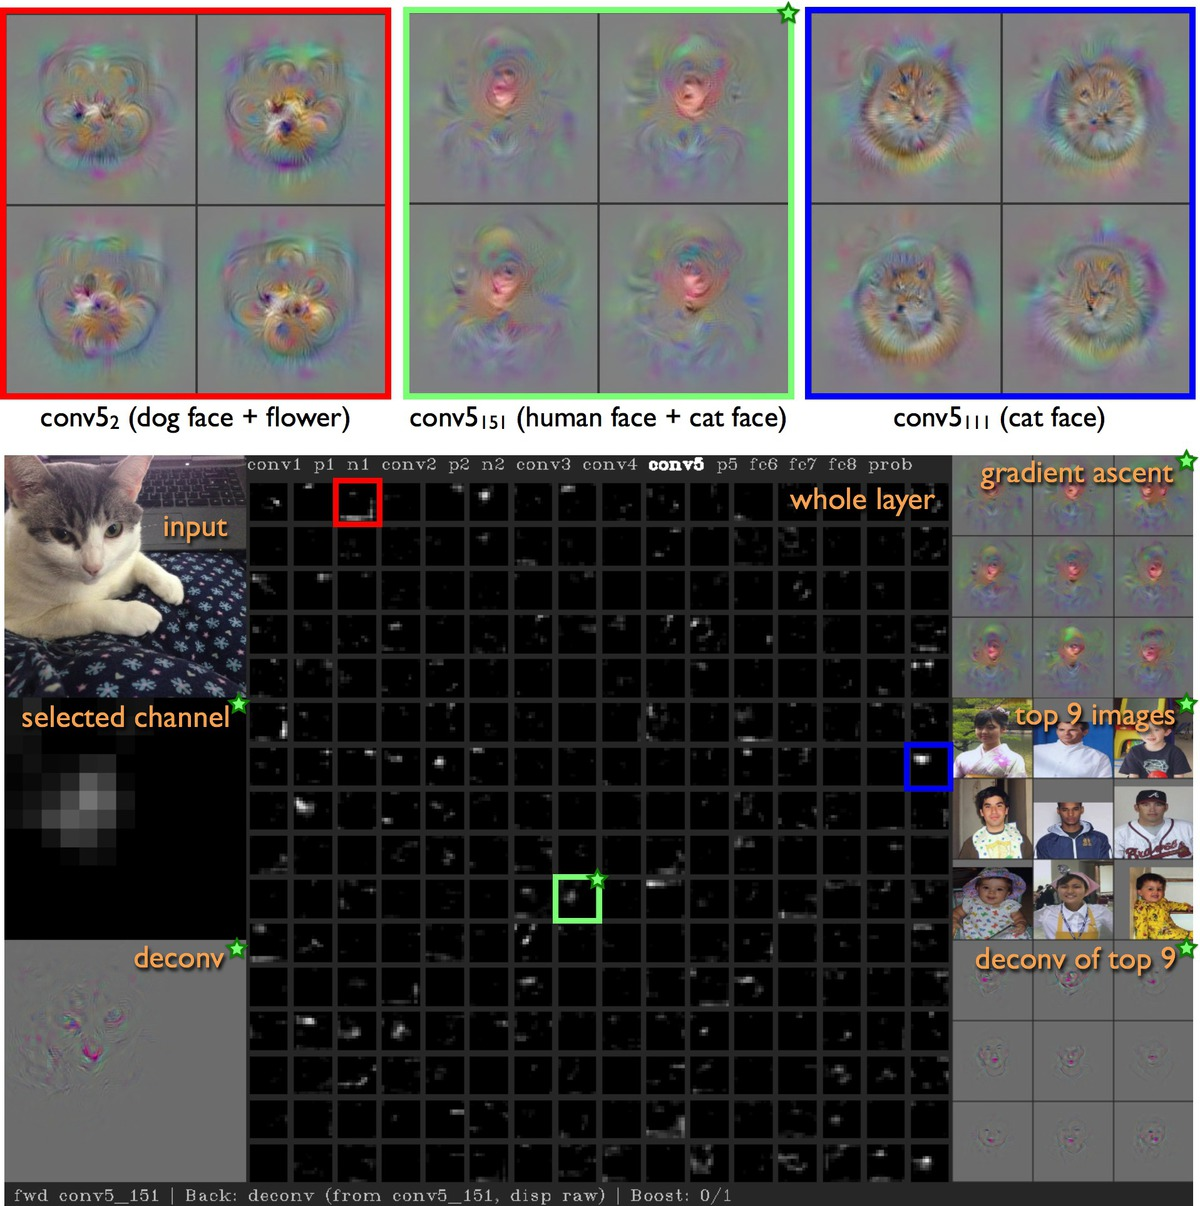
\includegraphics[width=0.7\linewidth]{\picPath/DVF_ex.png}
\end{center}
  \caption{Интерфейс программы Deep Visualization Framework.}
  \label{pic:DVF}
\end{figure}
\subsubsection{Визуализация активаций}
Каждый конволюционный и полносвязный слой Н.С. в результате работы передает следующему слою Feature Map, тензор вида $(B,H,W,C)$ для сверток и $(B,C)$ для полносвязных слоев, где $B $  - размер батча, $H, W$ - ширина и высота соответсвующей feature map и  $C$ - количество каналов. Для визуализации используется одно изображение ($B=1$) и карты активаций $(1,H,W,i)$ визуализируются для всех $i = \overline{1,C}$. На рисунке \ref{pic:DVF} область визуализации активаций обозначена как whole layer. Интерпретировать feature map можно как геометрическую карту, каждый элемент которой отвечает некоторой области входного изображения. Значение feature map в какой-то точке $(1,h,w,c)$  есть результат применения канала $c$ выбранной конволюции к области исходного изображения, отвечающей точке карты активации $(h,w)$. Таким образом яркие области feature map отечают областям исходного изображения, на которые среагировал заданный канал свертки. На рисунке \ref{pic:activations} изображена одна из карт активаций, сопоставленная с исходным изображением. Видно, что выбранная карта активизируется на областях, на которых присутствуют лица или даже морды животных.
\begin{figure}[H]
\begin{center}
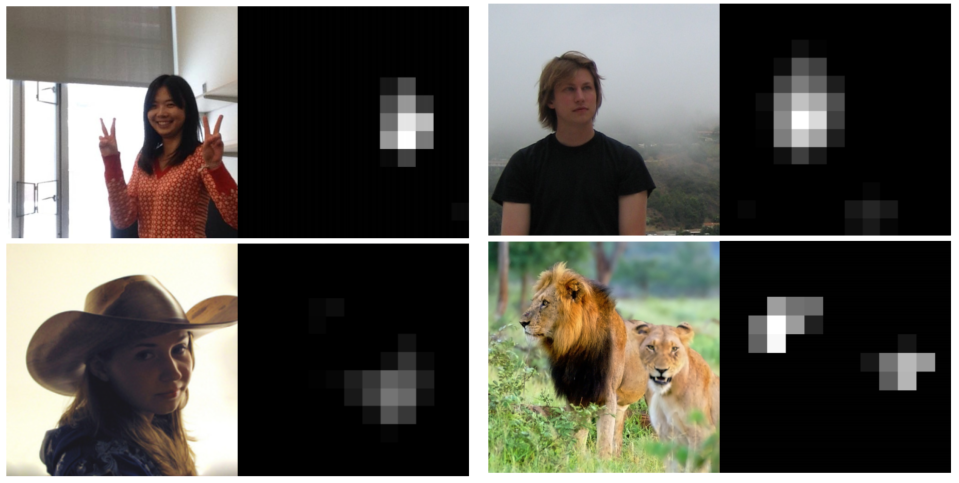
\includegraphics[width=0.8\linewidth]{\picPath/activations.png}
\end{center}
  \caption{Визуализация одного из каналов активаций сверточной нейронной сети, сопоставленная с исходным изображением. Видно, что выбранный канал имеет яркие области в местах, соответсвующих областям лиц}
  \label{pic:activations}
\end{figure}
\subsubsection{Градиентый подъем}
Градиентный подъем (gradient ascent) - метод, строющий входное изображение, максимизирующий выход выбранного канала. Для реализации на первом шаге фиксируется входное изображение - многоканальный белый шум и фиксируются все веса исследуемой сети. Производится тренировка сети т.е. forward pass и backward pass, но обучаемыми парамметрами являются только пиксели изображения. Однако если не использовать никаких регуляризаций, изображение после тренировки сложно интерпретировать так как оно мало отличается от случайного шума. Авторы Deep Visualisation Framework предлагают набор регуляризаций, который позволяет получать более интерпретируемые изображения. В частности даже $L_2$ норма делает изображение гороздо понятнее для человека. На рисунке \ref{pic:DVF} результаты градиентного подъема обозначены как gradient ascent.
\subsubsection{Деконволюция}
https://link.springer.com/content/pdf/10.1007%2F978-3-319-10590-1_53.pdf
Метод деконволюции - один из способов реализации функции, обратной к конволюционной нейронной сети. 
%пытается восстановить входное изображение по выходу сети, восстанавливая таким образом часть изображения, на которую опиралась конволюционная сеть во время принятия решения.
Реализация основывается на построении деконволюционной модели, состоящей также из сверток и пулинг слоев, имеющих те же веса, что и в исследуемой конволюционной модели. Однако деконволюционная модель на вход получает выход коволюционной сети и выдает изображение. Операции активации и пулинга не являются обратимыми, поэтому для реалзации обратной к конволюции функции используются значения, полученные во время прямого хода модели (switches)[] Для maxpool слоя, например, результатом инверсии является позиция максимального значения карты признаков предыдущего слоя.  

Чтобы исследовать работы конволюционной нейросети,  к каждому её слою присоединяется аналог обратной функции этого слоя, таким образом обеспечивая непрерывный путь от результатов модели к пикселям изображения. Для начала, входное изображение передается исходной сети, и для каждого слоя вычисляется функция активации. Чтобы получить обратное изображение, на последнем слое все активации, кроме целевой, зануляются, и значение активации передается в деконволюционную сеть, которая и выдает результирующее изображение. Результат деконволюции можно интерпретировать как области интереса исследуемой сети. На рисунке \ref{pic:DVF} деконволюция обозначена как deconv. Слева, в сравнении с исходным изображением видно, что область интереса сети для выбранного класса - морда кота. В то же время изображение клавиатуры на фоне никак не влияет на решение модели. 
\subsection{Улучшение деконволюции: Guided backpropogation}
Для визуализации конволюционных нейронных сетей в качестве основы авторы[] использовали подход деконволюции, однако привнесли некоторые улучшения.    
Процесс деконволюции можно описать следующим образом: На основе карты признаков исследуемого слоя, deconvnet пытается инвертировать операции каждого слоя, транслируя выход сети в исходное изображение. Однако для необратимых операций для псевдоинвертирования используются значения feature map прямого хода модели. Это делает метод деконволюции зависимым от входного изображения, и метод guided deconvolution позволяет избавиться от этой зависимости, получая более интерпретируемый результат. Это достигается путем простого удаления pooling слоев из классификационной модели.  Сравнение результатов с методом деконволюции можно увидеть на рисунке \ref{pic:g_backprop}
https://arxiv.org/pdf/1412.6806.pdf

\begin{figure}[H]
\begin{center}
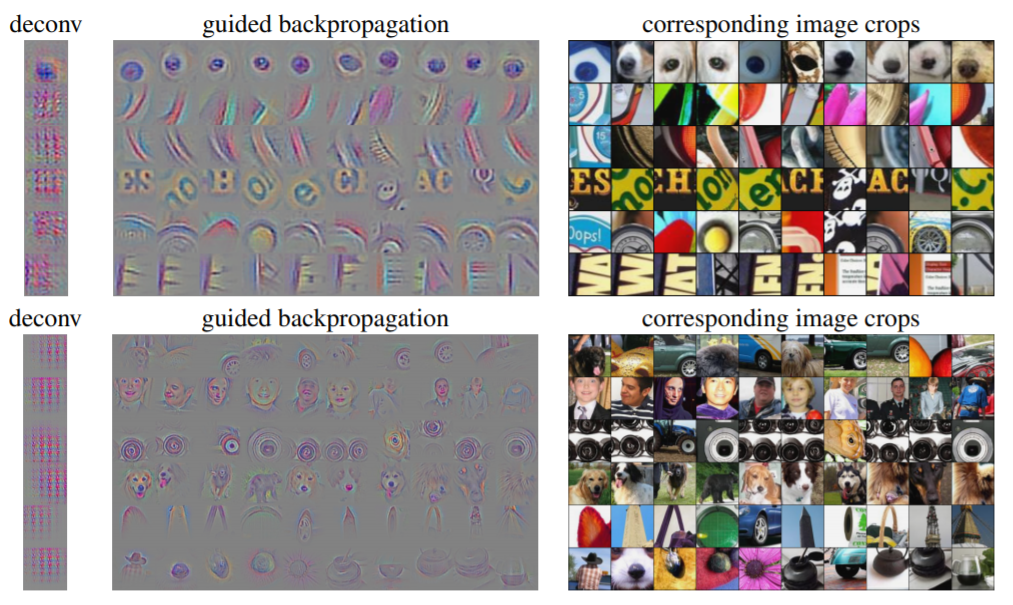
\includegraphics[width=0.8\linewidth]{\picPath/guided_backprop.png}
\end{center}
  \caption{Сравнение результатов визуализации guided backprop и деконволюции}
  \label{pic:g_backprop}
\end{figure}
Процесс визуализации giuded backprop описан на рисунке 
\ref{pic:g_backprop_scheme}. Сначала выбирается входное изображение и в сети выбирается нейрон или слой активации, работу которого необходимо визуализировать. Сеть производит прямой ход до слоя, в котором присутствует выбранная активация.  В этом слое зануляются все нейроны и слои, за исключением выбранных в начале. С выбранного слоя производится градиентный спуск, однако по ходу движения назад градиенты последовательно зануляются. Обозначая за $f^l$- слой начала градиентного спуска, градиенты предыдущих слоев вычисляются как $\frac{\partial f^{l}}{\partial f^{k}}_{guided}=\frac{\partial f^{l}}{\partial f^{k+1}}_{guided} \cdot max(0,\frac{\partial f^{k+1}}{\partial f^k})$ 
\begin{figure}[H]
\begin{center}
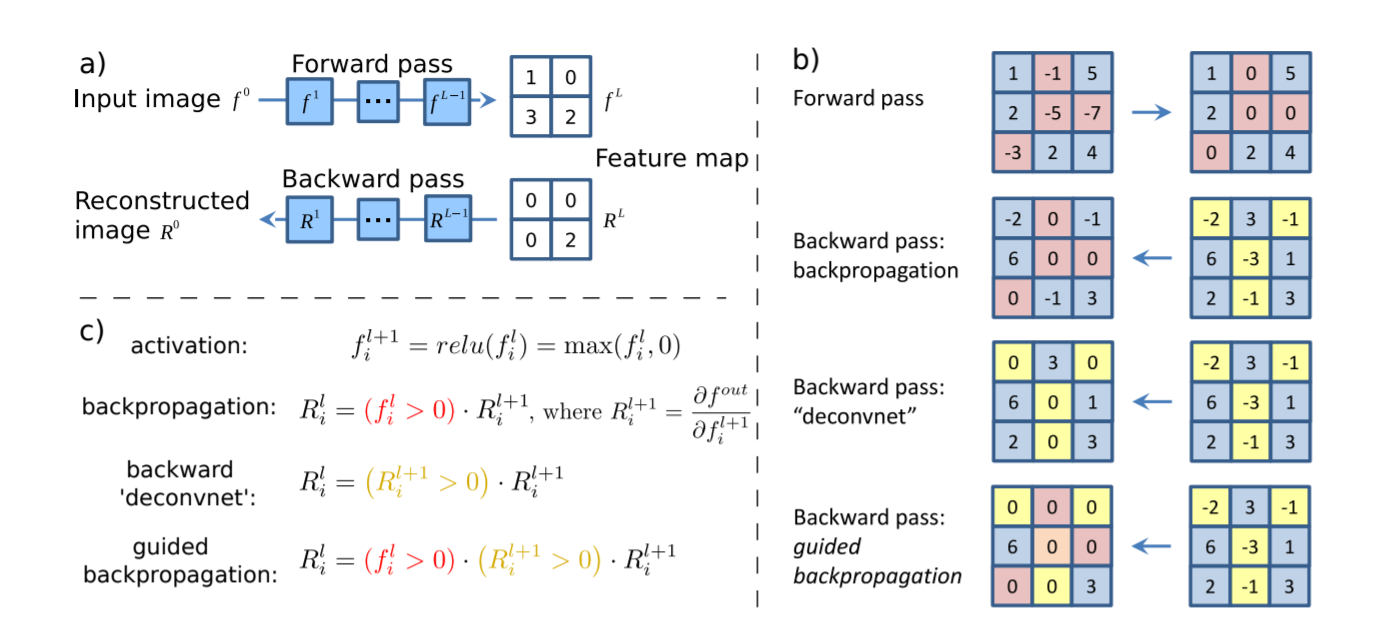
\includegraphics[width=0.8\linewidth]{\picPath/guided_backprop_scheme.png}
\end{center}
  \caption{Принцип работы метода guided backpropogation в отличие от деконволюции}
  \label{pic:g_backprop_scheme}
\end{figure}

Достоинством метода guided backprop является значительные улучшения результатов визуализации в сравнении с деконволюцией. Однако этот метод фиксирует архитектуру моделей, с которой может работать и не так эффективен как метод, описанный в следующей главе. 
\subsection{Grad Cam}
Относительно современный метод визуализации работы конволюционных сетей, не зависящий от наличия пулинг слоев и задачи классификации.  Gradcam предполагает наличие в конце модели полносвязного слоя, каждый нейрон которого отвечает за предсказание одного из результирующих классов.  На практике большинство конволюционных сетей, будь то сети классификации изображений или звуков, или даже сети, решающие задачу детектирования объектов, состоят из двух частей: головы (head) и шеи (backbone). Суть разделения заключается в том, что исходные данные путем прямого хода backbone части переводятся в латентное пространство признаков, являющиеся, по сути, областю определения head части модели. Такой подход удобен тем, что для разных задач для изображений (классификация, детектирование, сегментирование) можно использовать одну и ту же backbone часть модели. Метод GradCam использует карту признаков последнего конволюционного слой backbone части модели для визуализации работы всей модели. 
\begin{figure}[H]
\begin{center}
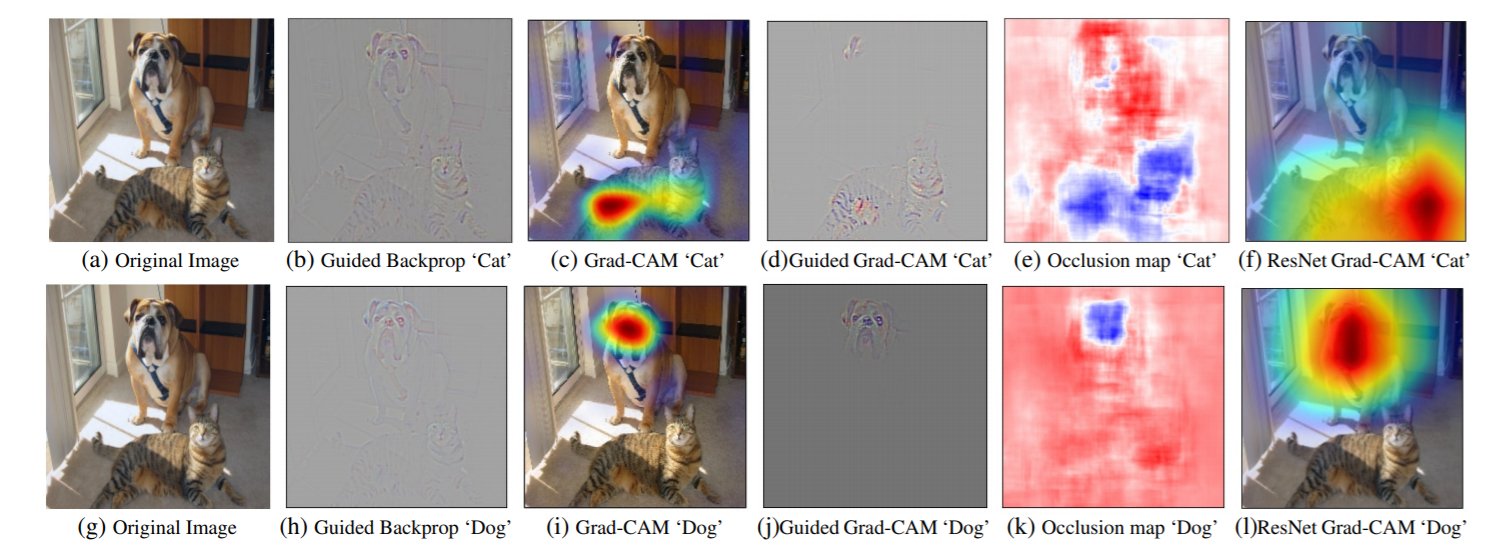
\includegraphics[width=\linewidth]{\picPath/gc_cat_and_dog.png}
\end{center}
  \caption{Сравнение методов визуализации классификации с методом визуализации grad cam}
  \label{pic:gc_cat_and_dog}
\end{figure}
Введем обозначения: $A^k \in R^{u \times v}, k 
\in K$ - карта признаков под номером $k$ самого глубокого слоя backbone части сети, $y^c$ - выход последнего полносвязного слоя, отвечающий за класс $c$ . Чтобы получить карту интереса сети для выбранного изображения I методом GradCam $L_{Grad=CAM}^c \in R^{u \times v}$ шириной $u$ и высотой $v$ для класса $c$ необходимо произвести прямой ход модели на изображении I до финального полносвязного слоя, и вычислить градиеты $\frac{\partial y^c}{\partial A_{i,j}^k}, \forall k \in K$. Далее на основе этой информации вычисляется весовой коэффициент для каждой карты признаков $A^k$:
$$
\alpha_k^c  = \frac{1}{u+v}\sum_{i = 1}^u 
\sum_{j=1}^v \frac{\partial y^c}{\partial A_{i,j}^k}
$$
Что по сути является усредненным значением градиенты в выбранной карте признаков. Финальная визуализация вычисляется по формуле:
$$
L^c_{Grad-CAM} = ReLU(\sum_{k \in K} \alpha_k^c A^k)
$$
Функция $ReLU$ используется для исключения элементов визуализации, вносящих отрицательный вес в предсказании выбранного класса. После этого полученная визуализация равномерно растягивется на область всего изображения. Кроме того, метод gradCam можно объединить с  методом Визуализацию этого процесса можно наблюдать на изображении \ref{pic:gc_cat_and_dog}. 

\begin{figure}[H]
\begin{center}
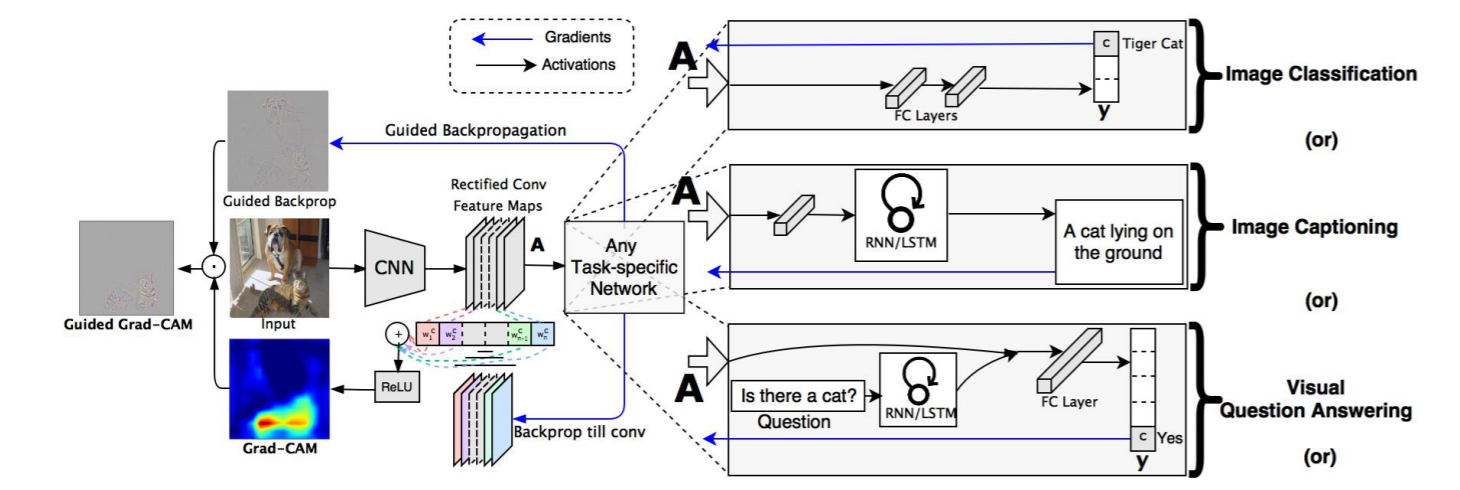
\includegraphics[width=1.1\linewidth]{\picPath/gc_sheme.png}
\end{center}
  \caption{Принцип работы метода GradCam}
  \label{pic:gc_cat_and_dog}
\end{figure}
Метод визуализации GradCam прост в реализации нетребователен к архитектуре моделей, что делает его хорошим кандидатом для визуализации работы конволюционных сетей.

\chapter{Проблема классификации ЭКГ}
\section{Обзор проблемы}
Сердечно-сосудистые заболевания являются ведущей причиной смерти во всем мире, и электрокардиограмма (ЭКГ) является важным инструментом в их диагностике. По мере перехода ЭКГ с аналоговой на цифровую, автоматизированный компьютерный анализ стандартных электрокардиограмм в 12 каналах приобрел значение в процессе медицинской диагностики. Однако ограниченная производительность классических алгоритмов исключает его использование в качестве автономного диагностического инструмента и отводит им вспомогательную роль.[https://www.nature.com/articles/s41467-020-15432-4]

Кратковременная стандартная ЭКГ в 12 каналов (S12L-ECG) - это наиболее часто используемое дополнительное обследование для оценки состояния сердца, применяемое во всех клинических учреждениях, от центров первичной медико-санитарной помощи до отделений интенсивной терапии. В то время как долгосрочный мониторинг сердца, например, при холтеровском обследовании, дает информацию в основном о сердечном ритме и реполяризации, S12L-ЭКГ может предоставить полную оценку электрической активности сердца. В список классифицируемых болезней входят входят аритмии, нарушения проводимости, острые коронарные синдромы, гипертрофия и увеличение сердечной камеры и даже эффекты лекарств и электролитные нарушения.
[https://www.nature.com/articles/s41467-020-15432-4]

\section{Обзор датасета}
Набор данных ЭКГ PTB-XL - это большой набор данных из 21837 клинических ЭКГ в 12 отведениях от 18885 пациентов длительностью 10 секунд. Необработанные данные формы волны были аннотированы двумя кардиологами, которые присвоили каждой записи потенциально несколько отчетов ЭКГ. Всего 71 отчет ЭКГ соответствует стандарту SCP-ЭКГ и охватывает диагностические, формуляры и ритмические утверждения. Чтобы обеспечить сопоставимость алгоритмов машинного обучения, обученных на наборе данных, исследователи предоставляют рекомендуемые к использованию разбиения на обучающие и тестовые наборы. В сочетании с обширными аннотациями это превращает набор данных в богатый ресурс для обучения и оценки алгоритмов автоматической интерпретации ЭКГ. Набор данных дополняется обширными метаданными по демографическим характеристикам, характеристикам инфаркта, вероятности диагностических заявлений ЭКГ, а также аннотированными свойствами сигналов.

Данные, лежащие в основе набора данных ЭКГ PTB-XL, были собраны с помощью устройств компании Schiller AG в течение почти семи лет с октября 1989 года по июнь 1996 года. С приобретением оригинальной базы данных у Schiller AG полные права на использование были переданы Physikalisch-Technische Bundesanstalt (PTB). Записи были курированы и преобразованы в структурированную базу данных в рамках долгосрочного проекта в  PTB. База данных использовалась в ряде публикаций, но доступ к ней до сих пор оставался ограниченным. Комитет по институциональной этике одобрил публикацию анонимных данных в базе данных открытого доступа (PTB-2020-1). В ходе процесса публичного выпуска в 2019 году существующая база данных была оптимизирована для удобства использования и доступности сообществу машинного обучения. Данные ЭКГ и метаданные были преобразованы в открытые форматы данных, которые легко обрабатываются стандартным программным обеспечением.[https://doi.org/10.13026/x4td-x982.]
\section{Методы решения}
В течение последних 22 лет PhysioNet и Computing in Cardiology совместно организовали серию ежегодных соревнований для решения клинически интересных задач, которые либо не решены, либо не решены должным образом. В последний раз соревнование проходило в 2020 году, и в качестве основной архитектуры решения задачи классификации ЭКГ использовались конволюционные сети.[https://physionetchallenges.org/2020/][https://github.com/Bsingstad/PhysioNet-CinC-Challenge2020-TeamUIO]

В качестве модели классификации ЭКГ в этой работе используется модель Antônio H. Ribeiro[], имеющася в открытом доступе. В качестве ахитектуры была выбрана resnet  подобная одномерная сеть, арихтектура которой изображена на рисунке 
[ComputerECGerrors2007.pdf]
[https://www.researchgate.net/publication/327263145_Heartbeat_classification_fusing_temporal_and_morphological_information_of_ECGs_via_ensemble_of_classifiers]


\begin{figure}[H]
\begin{center}
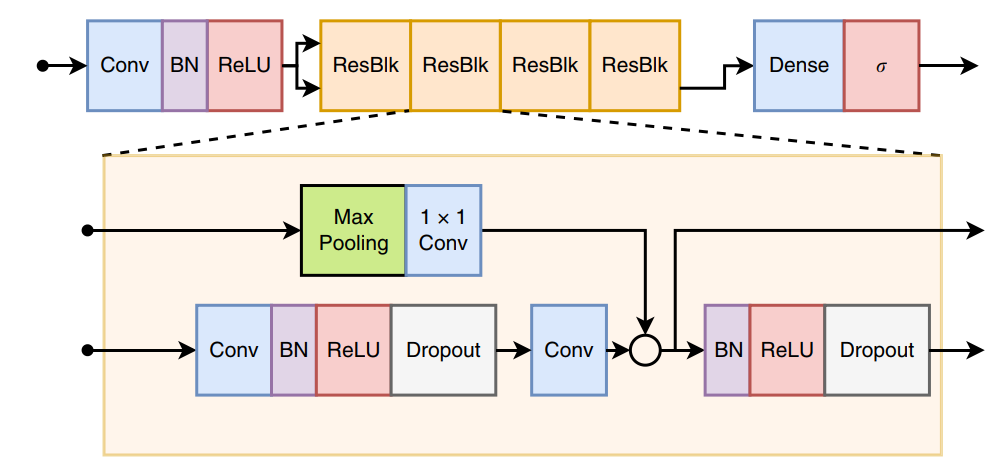
\includegraphics[width=0.8\linewidth]{\picPath/ecg_resnet.png}
\end{center}
  \caption{Архитектура модели классификации ЭКГ, предложенная  Antônio H. Ribeiro}
  \label{pic:ecg_resnet}
\end{figure}

\begin{figure}[H]
\begin{center}
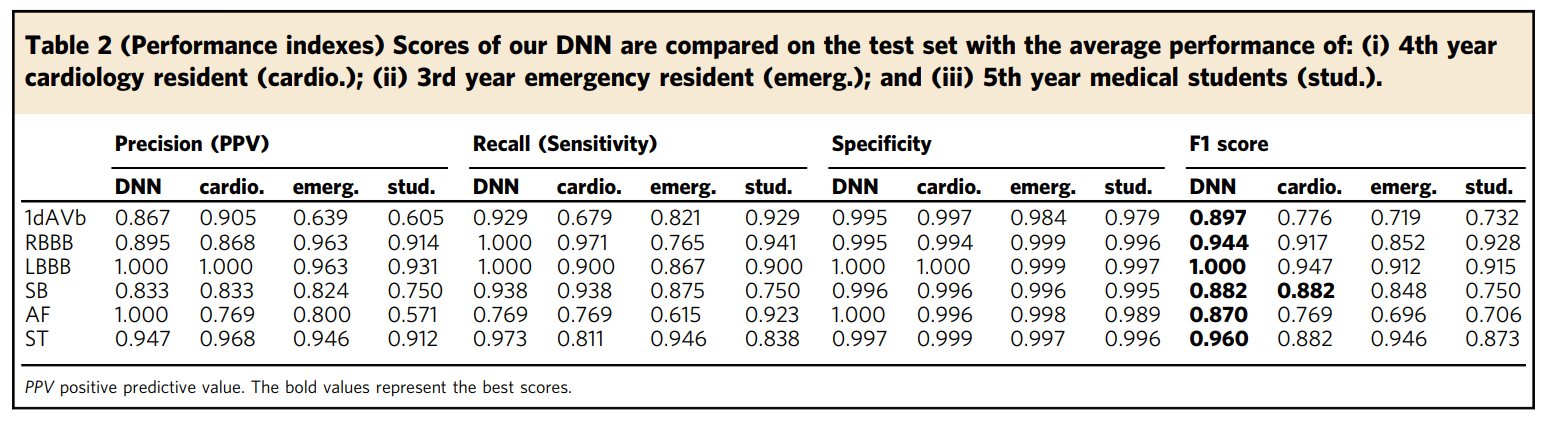
\includegraphics[width=1.1\linewidth]{\picPath/ecg_paper_res.png}
\end{center}
  \caption{Результаты валидации модели на тестовом датасете, предоставленном в статье}
  \label{pic:ecg_paper_res}
\end{figure}

Модель имеет хорошую точность на предоставленном тестовом датасете, однако имеет ряд недостатков: модель натренированна на закрытом датасете с 6 непересекающимися классами и использует одномерные сигналы разрешением 400Hz, хотя датасет  PTB-XL предоставляет данные в разрешении 500Hz и имеет порядка 30 классов. В рамках работы модель была протестированна на 5 разбиении PTB-XL на примерах, имеющих только допустимые наборы классов для модели из этой главы. Результаты работы, представленные в таблице \ref{tab:ecg_results}, показывают худший результат работы модели на новых данных.
\begin{table}[H]
% Подпись таблицы
\caption{Результаты валидации модели на  5 разбиении PTB-XL на примерах, имеющих только допустимые наборы классов}

\label{tab:ecg_results}
\begin{tabularx}{\textwidth}{|X|X|X|X|X|} % Столько X, сколько столбцов
\hline 
&precision & recall &  f1-score  &support \\ \hline
1dAVb   &    0.58   &   0.76  &    0.66  &      79 \\ \hline 
    RBBB   &     0.85   &    0.93   &    0.88  &       54 \\ \hline 
    LBBB   &    0.84   &   0.91   &   0.87   &     53 \\ \hline
      SB  &     0.89   &   0.66  &    0.76  &      64 \\ \hline
      AF    &   0.95  &    0.91  &    0.93   &    152 \\ \hline
      ST  &     0.86  &    0.90   &   0.88   & 83   \\ \hline
\end{tabularx}
\end{table}
\section{Способ визуализации результатов конволюционной сети: GradCam}
В качестве метода визуализации работы выбранной модели классификации выбран метод GradCam. В качестве входных изображений были взяты ЭКГ сигналы из датасета PTB-XL со следующими порядковыми номерами: 282, 424, 489, 1694, 19715, 21585. Эти кардиограммы относятся к разным  допустимым для модели классам и, кроме того, правильно классифицируются моделью. Метод GradCam предполагал наличие двумерной карты признаков, однако формула легко обобщается на одномерный случай. На рисунках   \ref{pic:282.png}- \ref{pic:21585.png}. Метод GradCam не разделяет входные каналы, поэтому карта интереса модели общая для всех 12 каналов. 

\begin{figure}[H]
\begin{center}
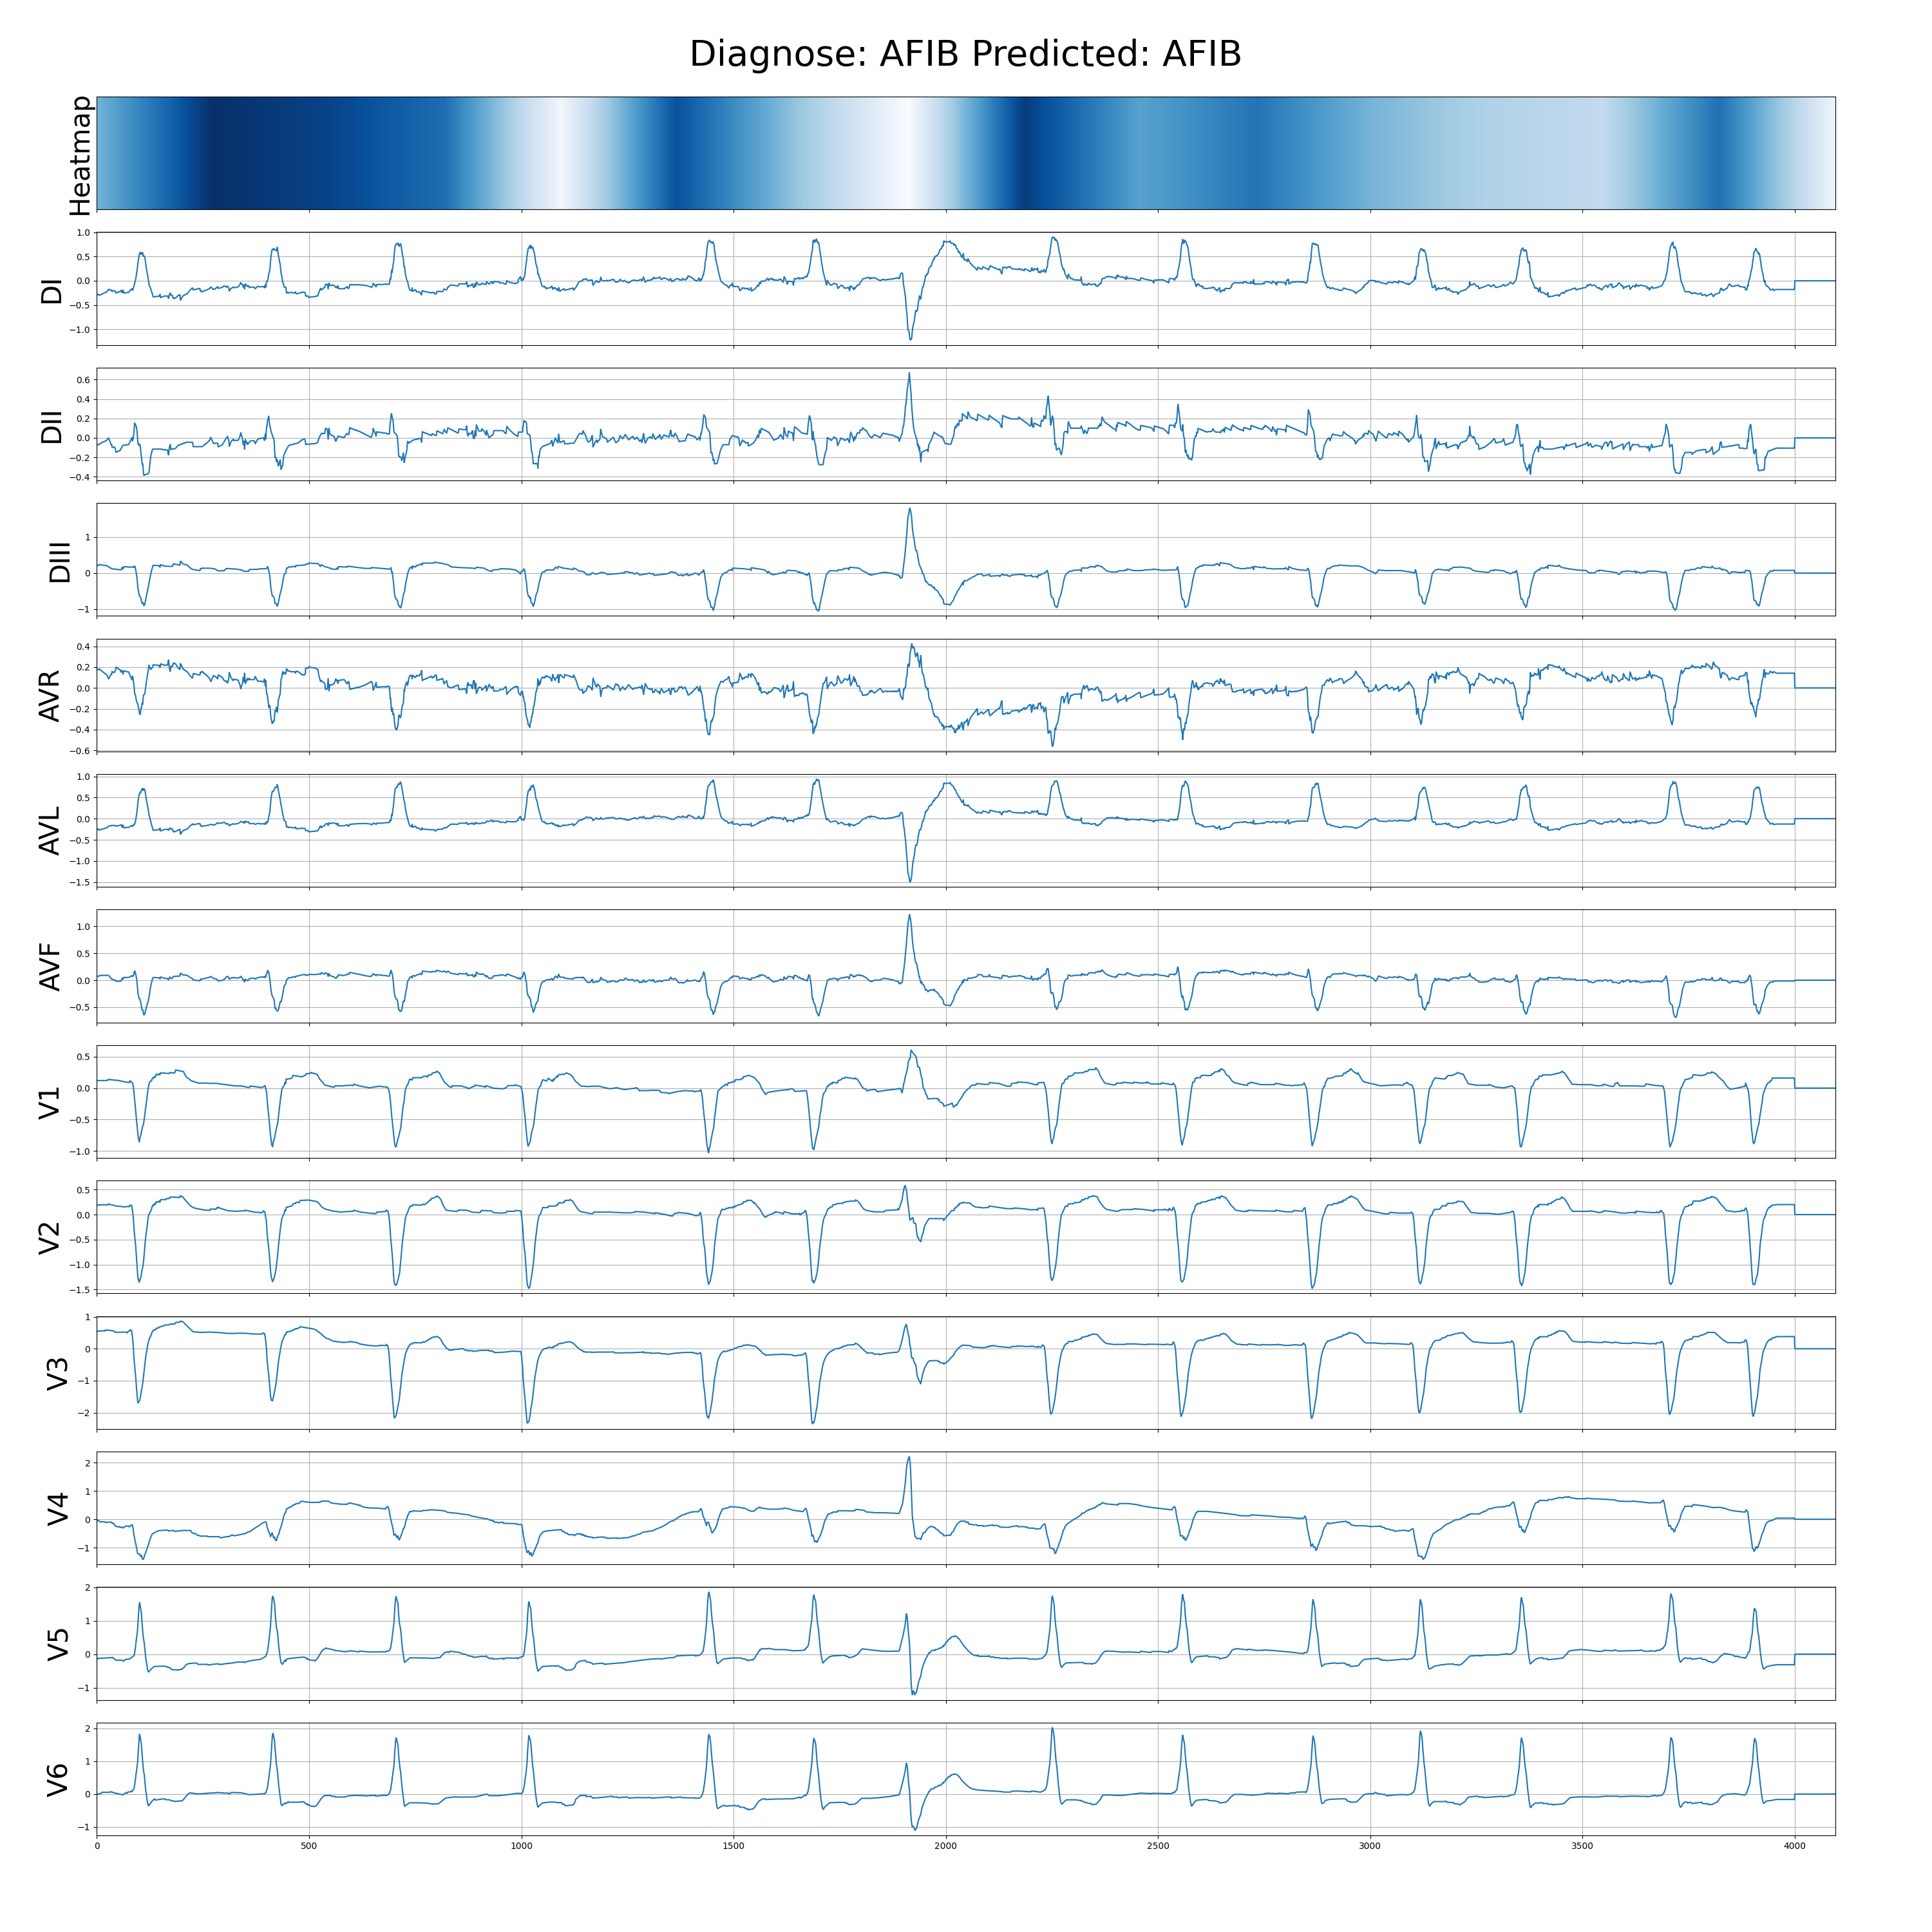
\includegraphics[width=1.1\linewidth]{\picPath/ecg_viz/282.png}
\end{center}
  \caption{Области внимания модели для ЭКГ сигнала с диагнозом "Мерцательная аритмия"}
  \label{pic:282.png}
\end{figure}
\newpage
\begin{figure}[H]
\begin{center}
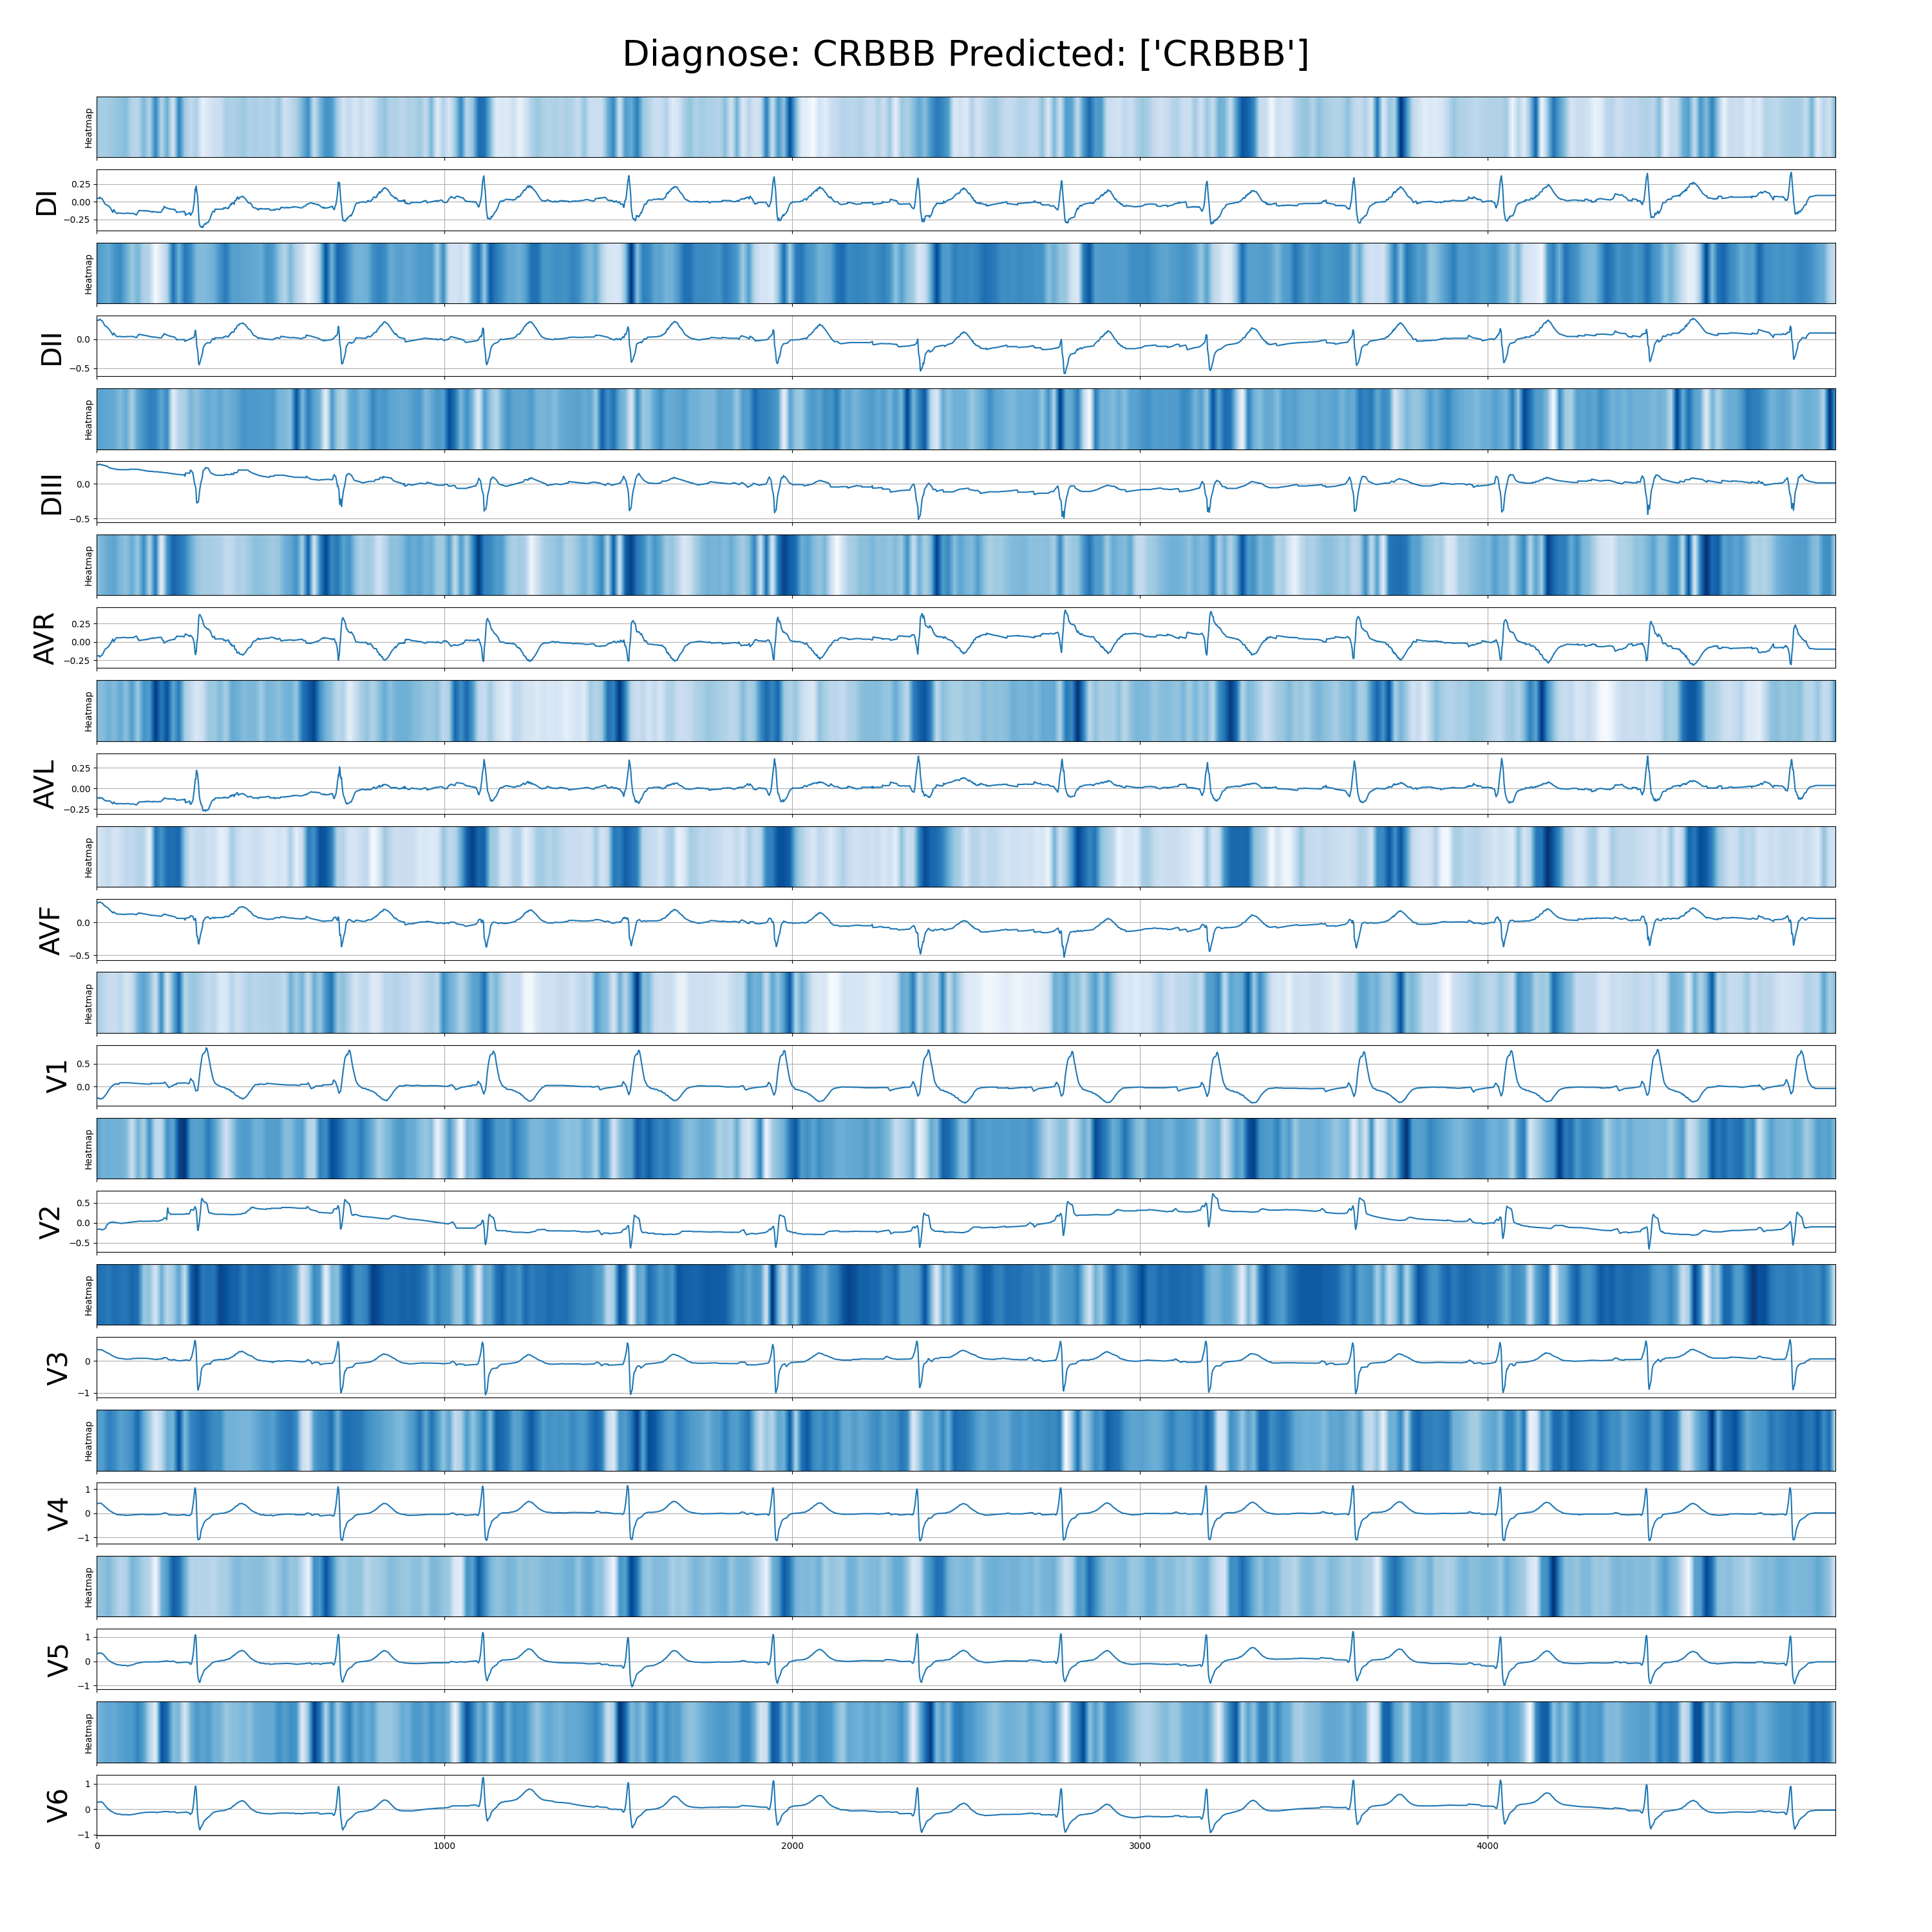
\includegraphics[width=1.1\linewidth]{\picPath/ecg_viz/424.png}
\end{center}
  \caption{Области внимания модели для ЭКГ сигнала с диагнозом "Блокада правой ножки пучка Гиса"}

\end{figure}
\newpage
\begin{figure}[H]
\begin{center}
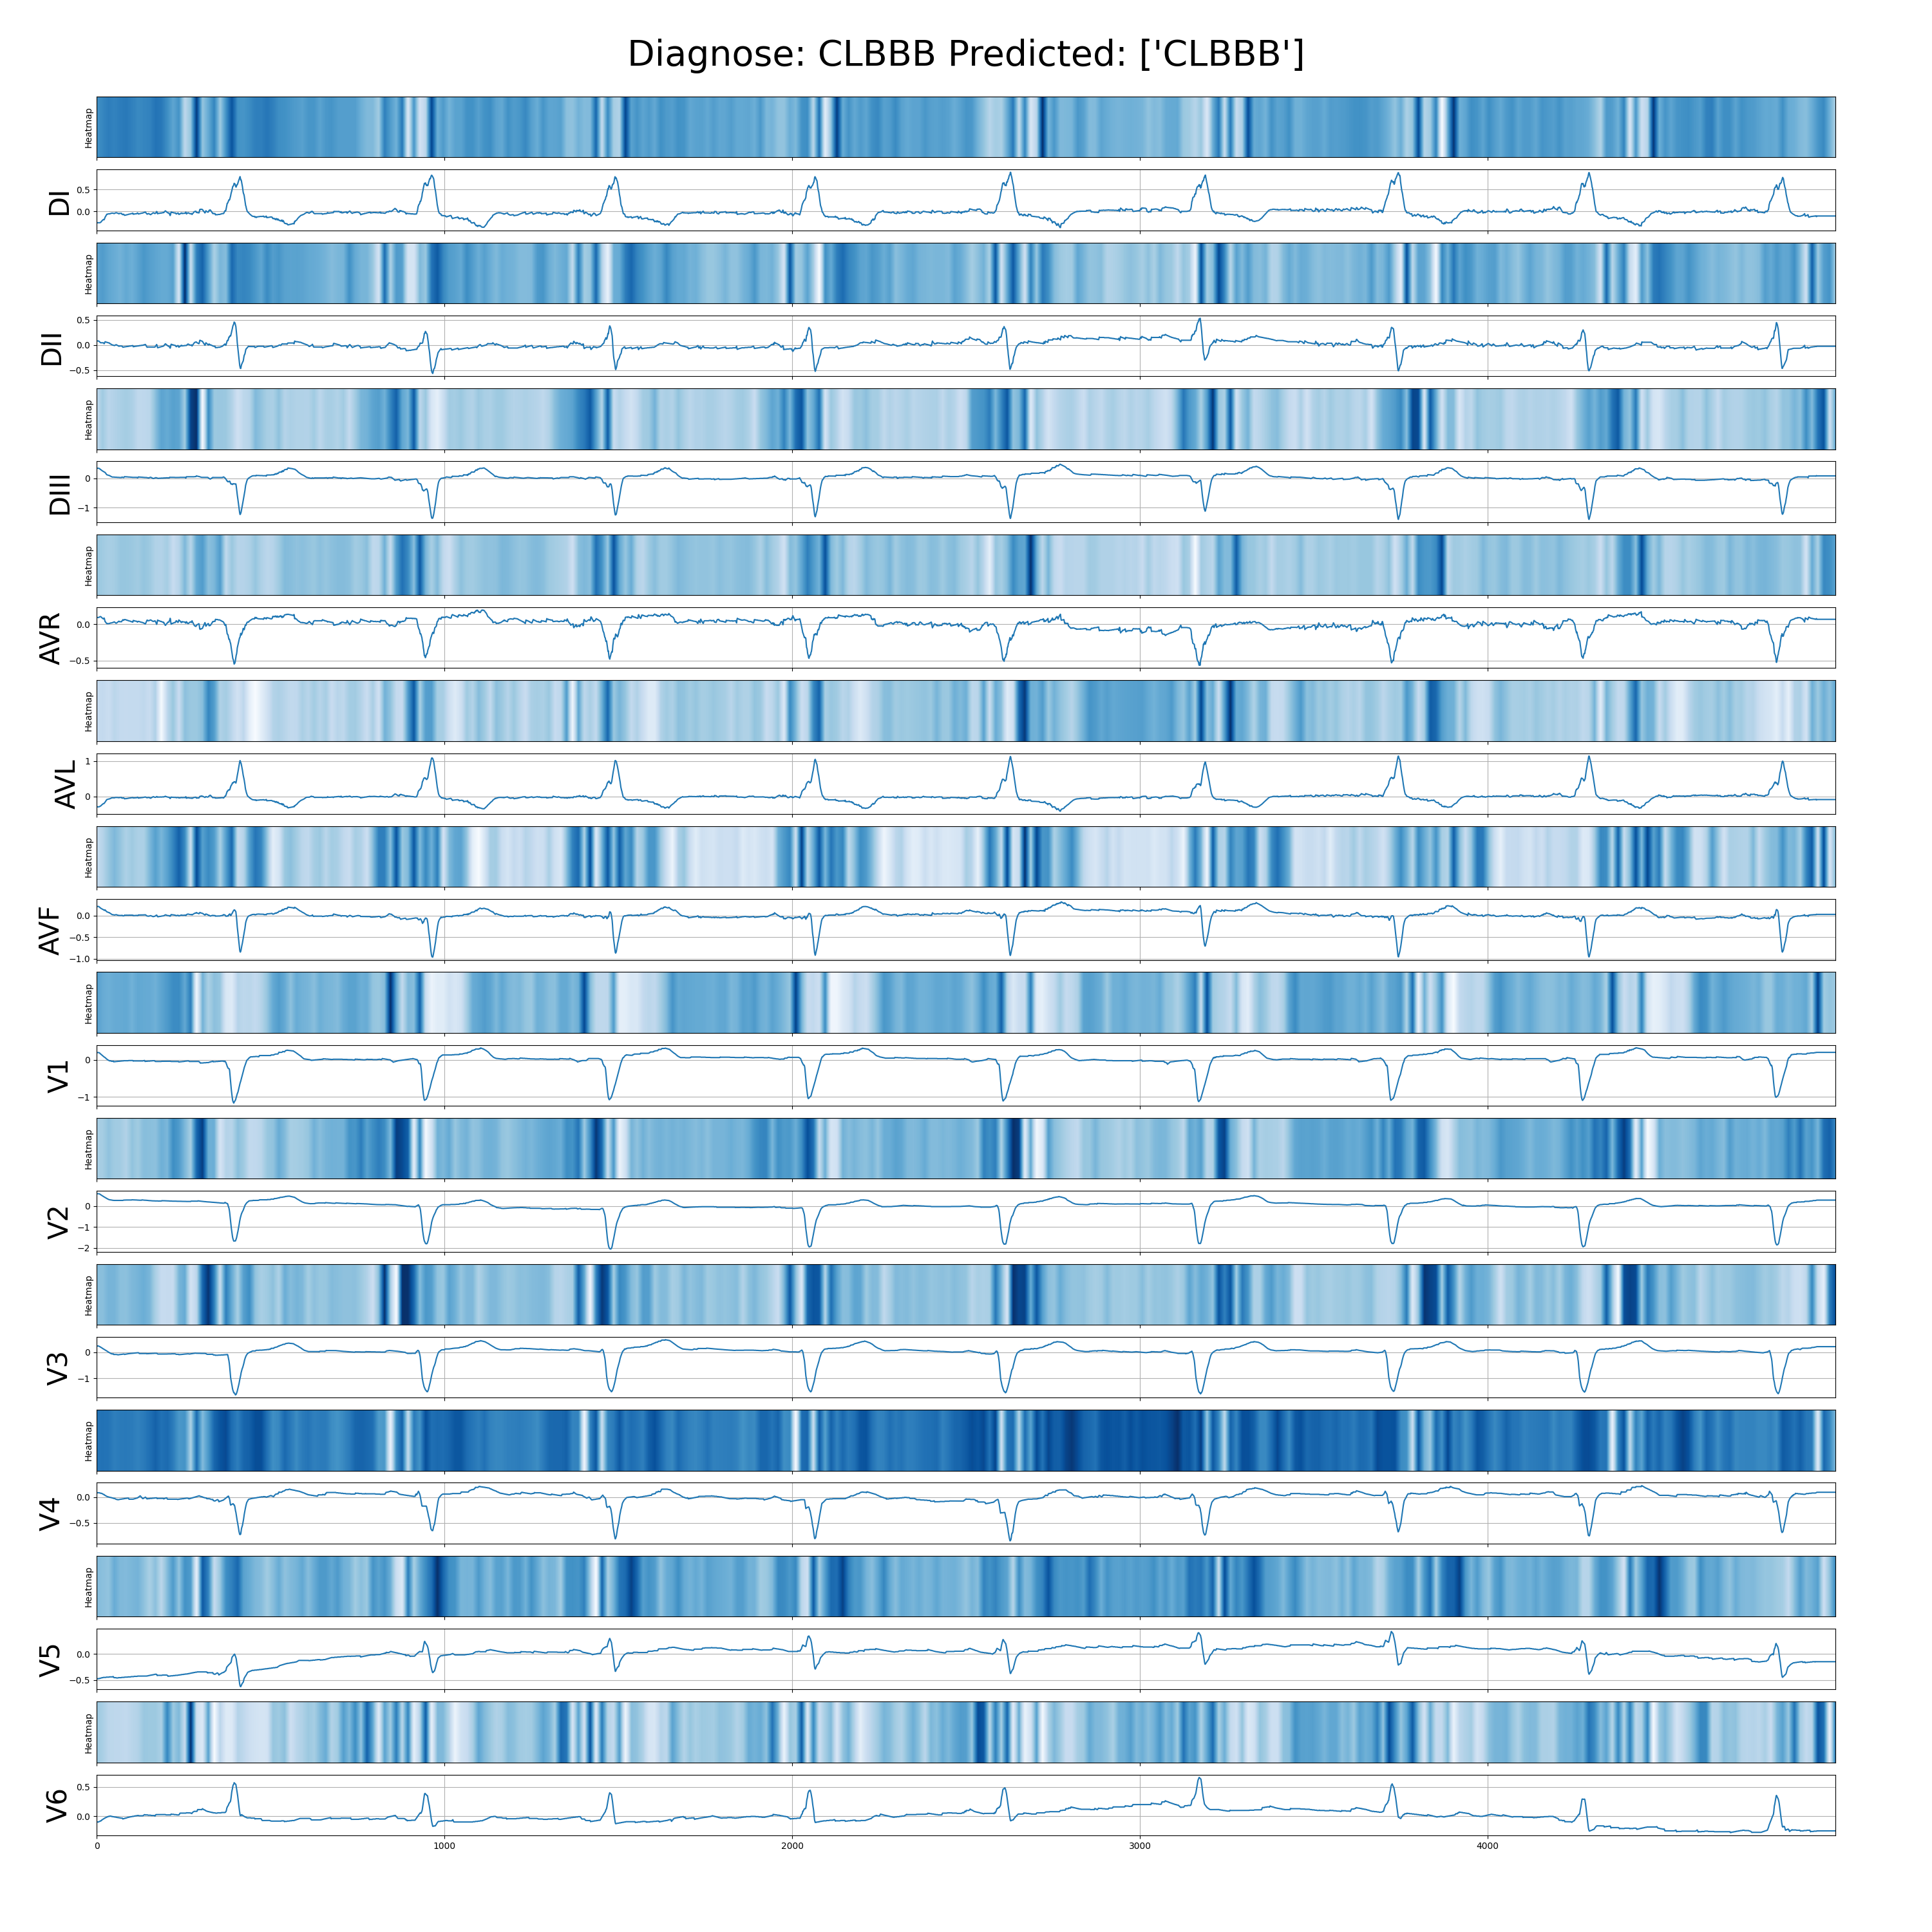
\includegraphics[width=1.1\linewidth]{\picPath/ecg_viz/489.png}
\end{center}
  \caption{Области внимания модели для ЭКГ сигнала с диагнозом "Блокада левой ножки пучка Гиса"}

\end{figure}
\newpage

\begin{figure}[H]
\begin{center}
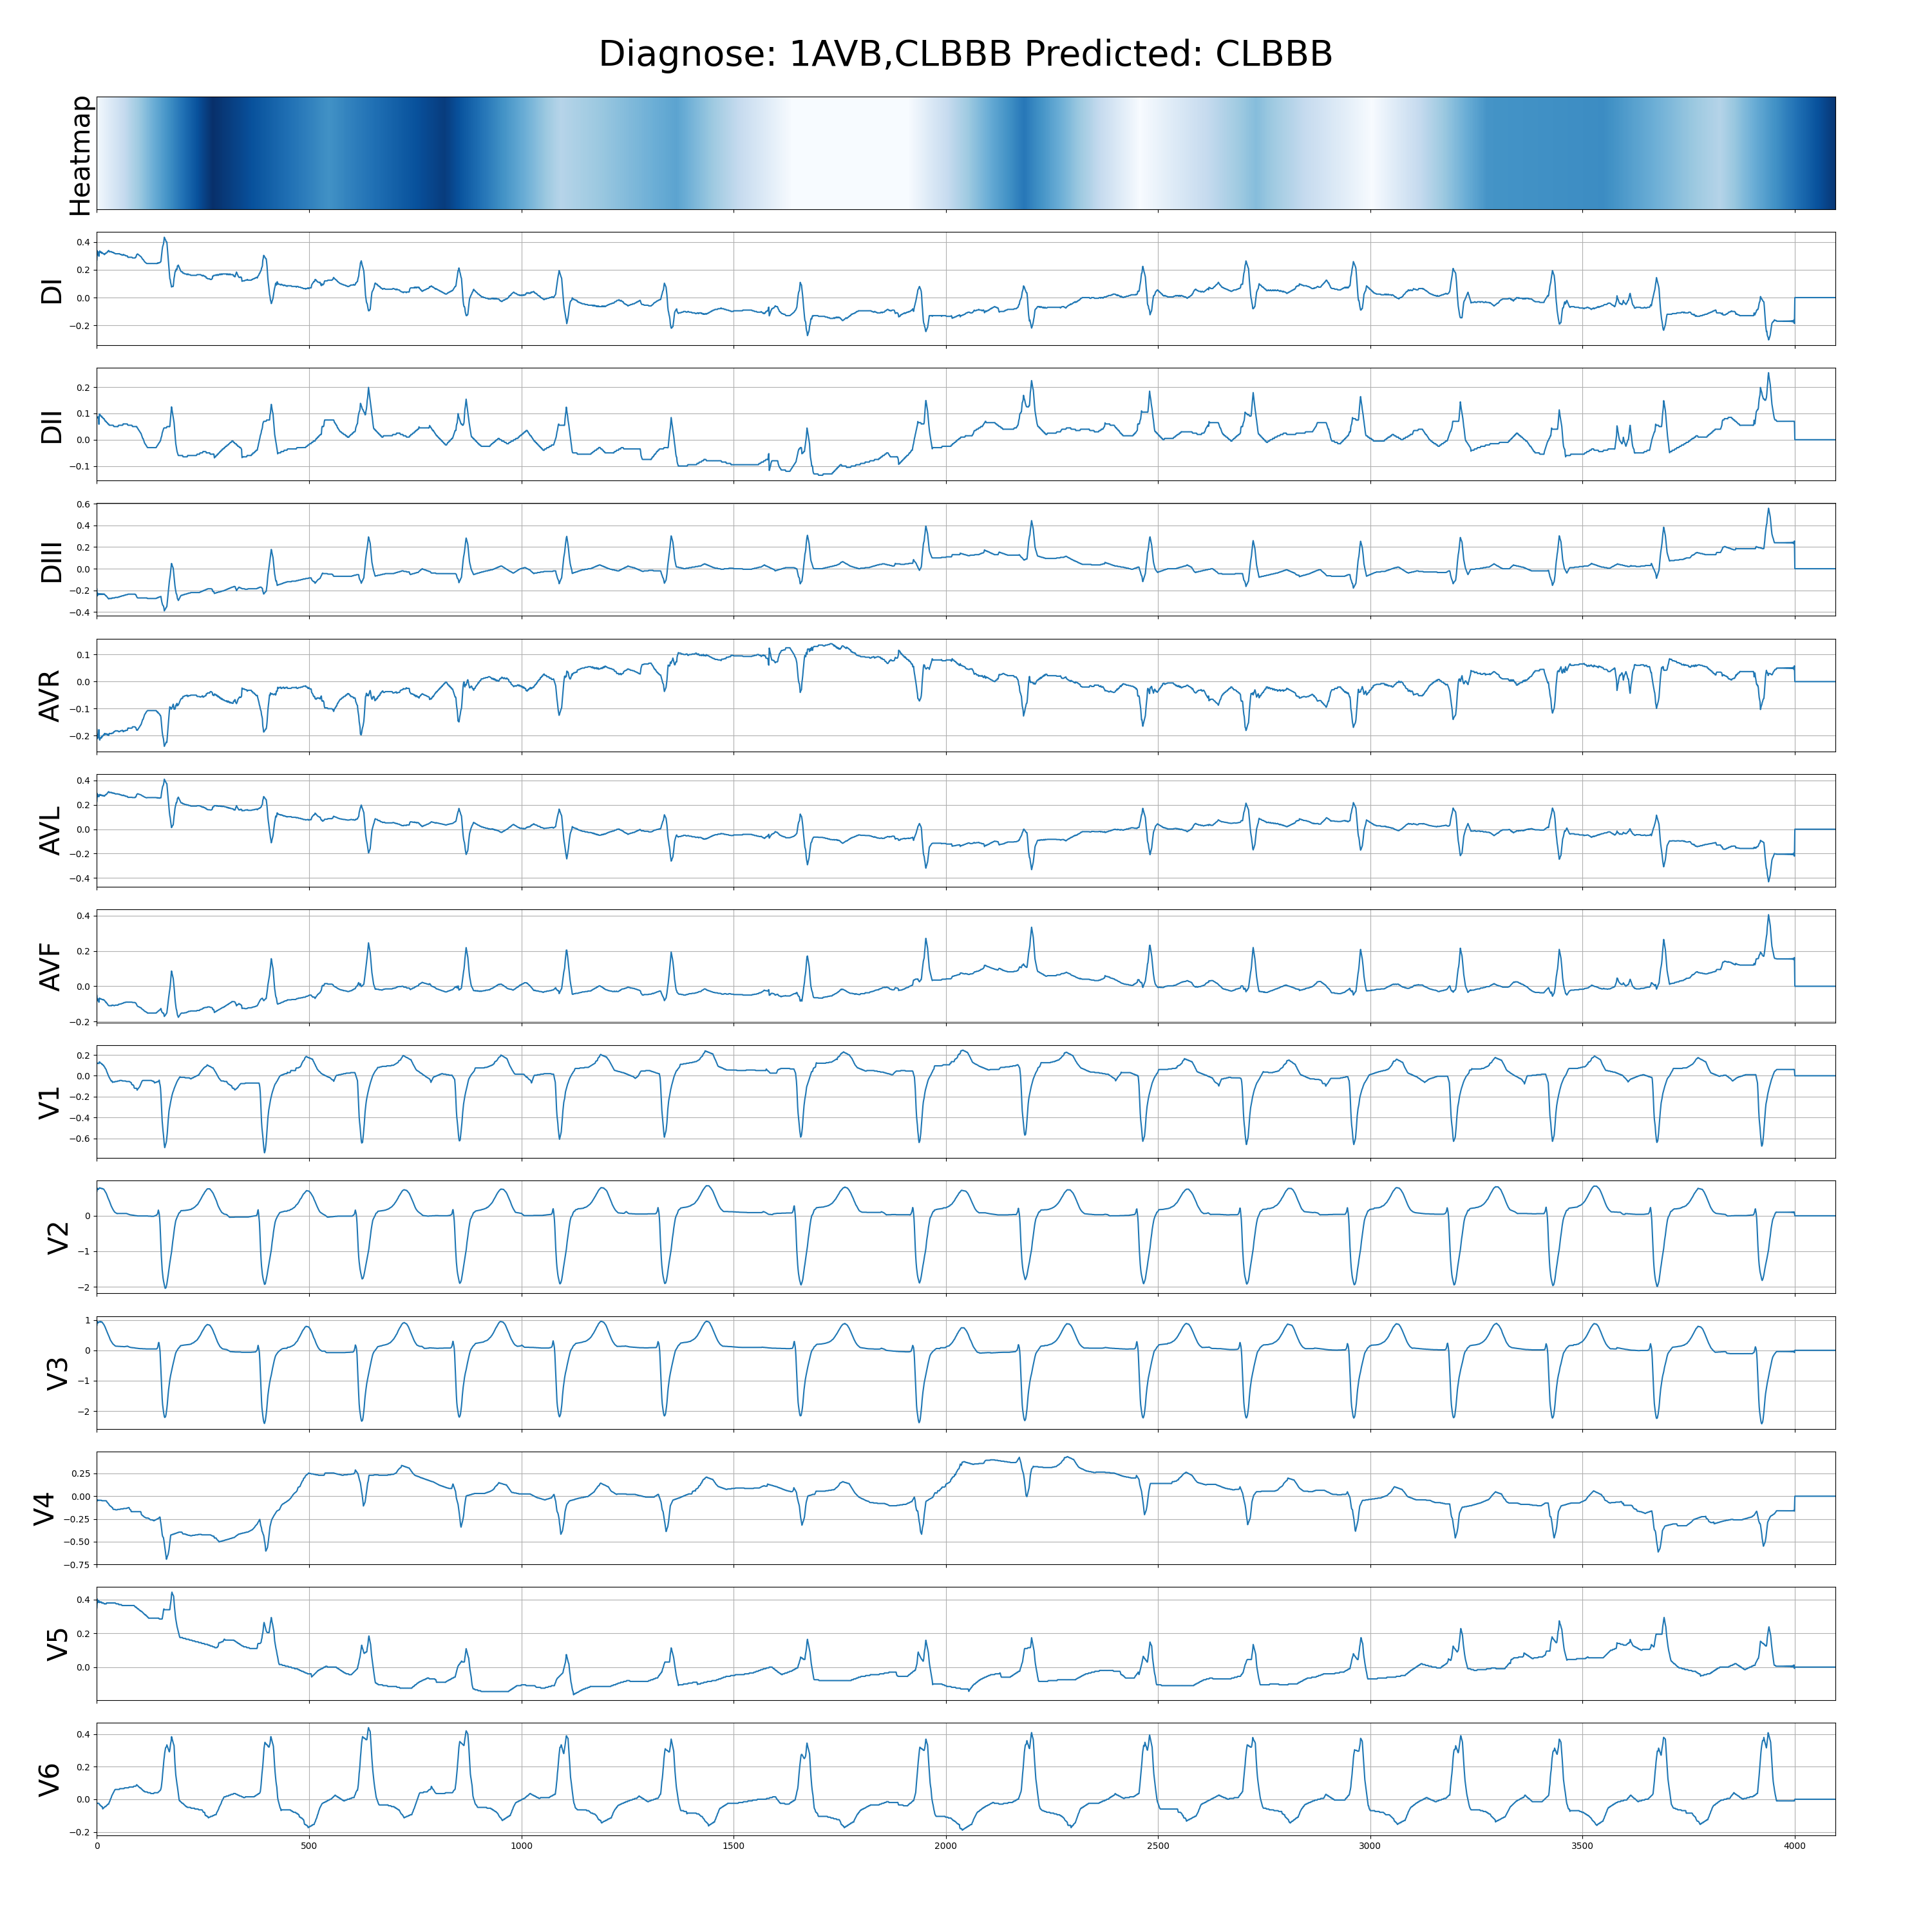
\includegraphics[width=1.1\linewidth]{\picPath/ecg_viz/1694.png}
\end{center}
  \caption{Области внимания модели для ЭКГ сигнала с диагнозом "Атриовентрикулярная блокада первой степени и блокада левой ножки пучка Гиса "}
  
\end{figure}
\newpage
\begin{figure}[H]
\begin{center}
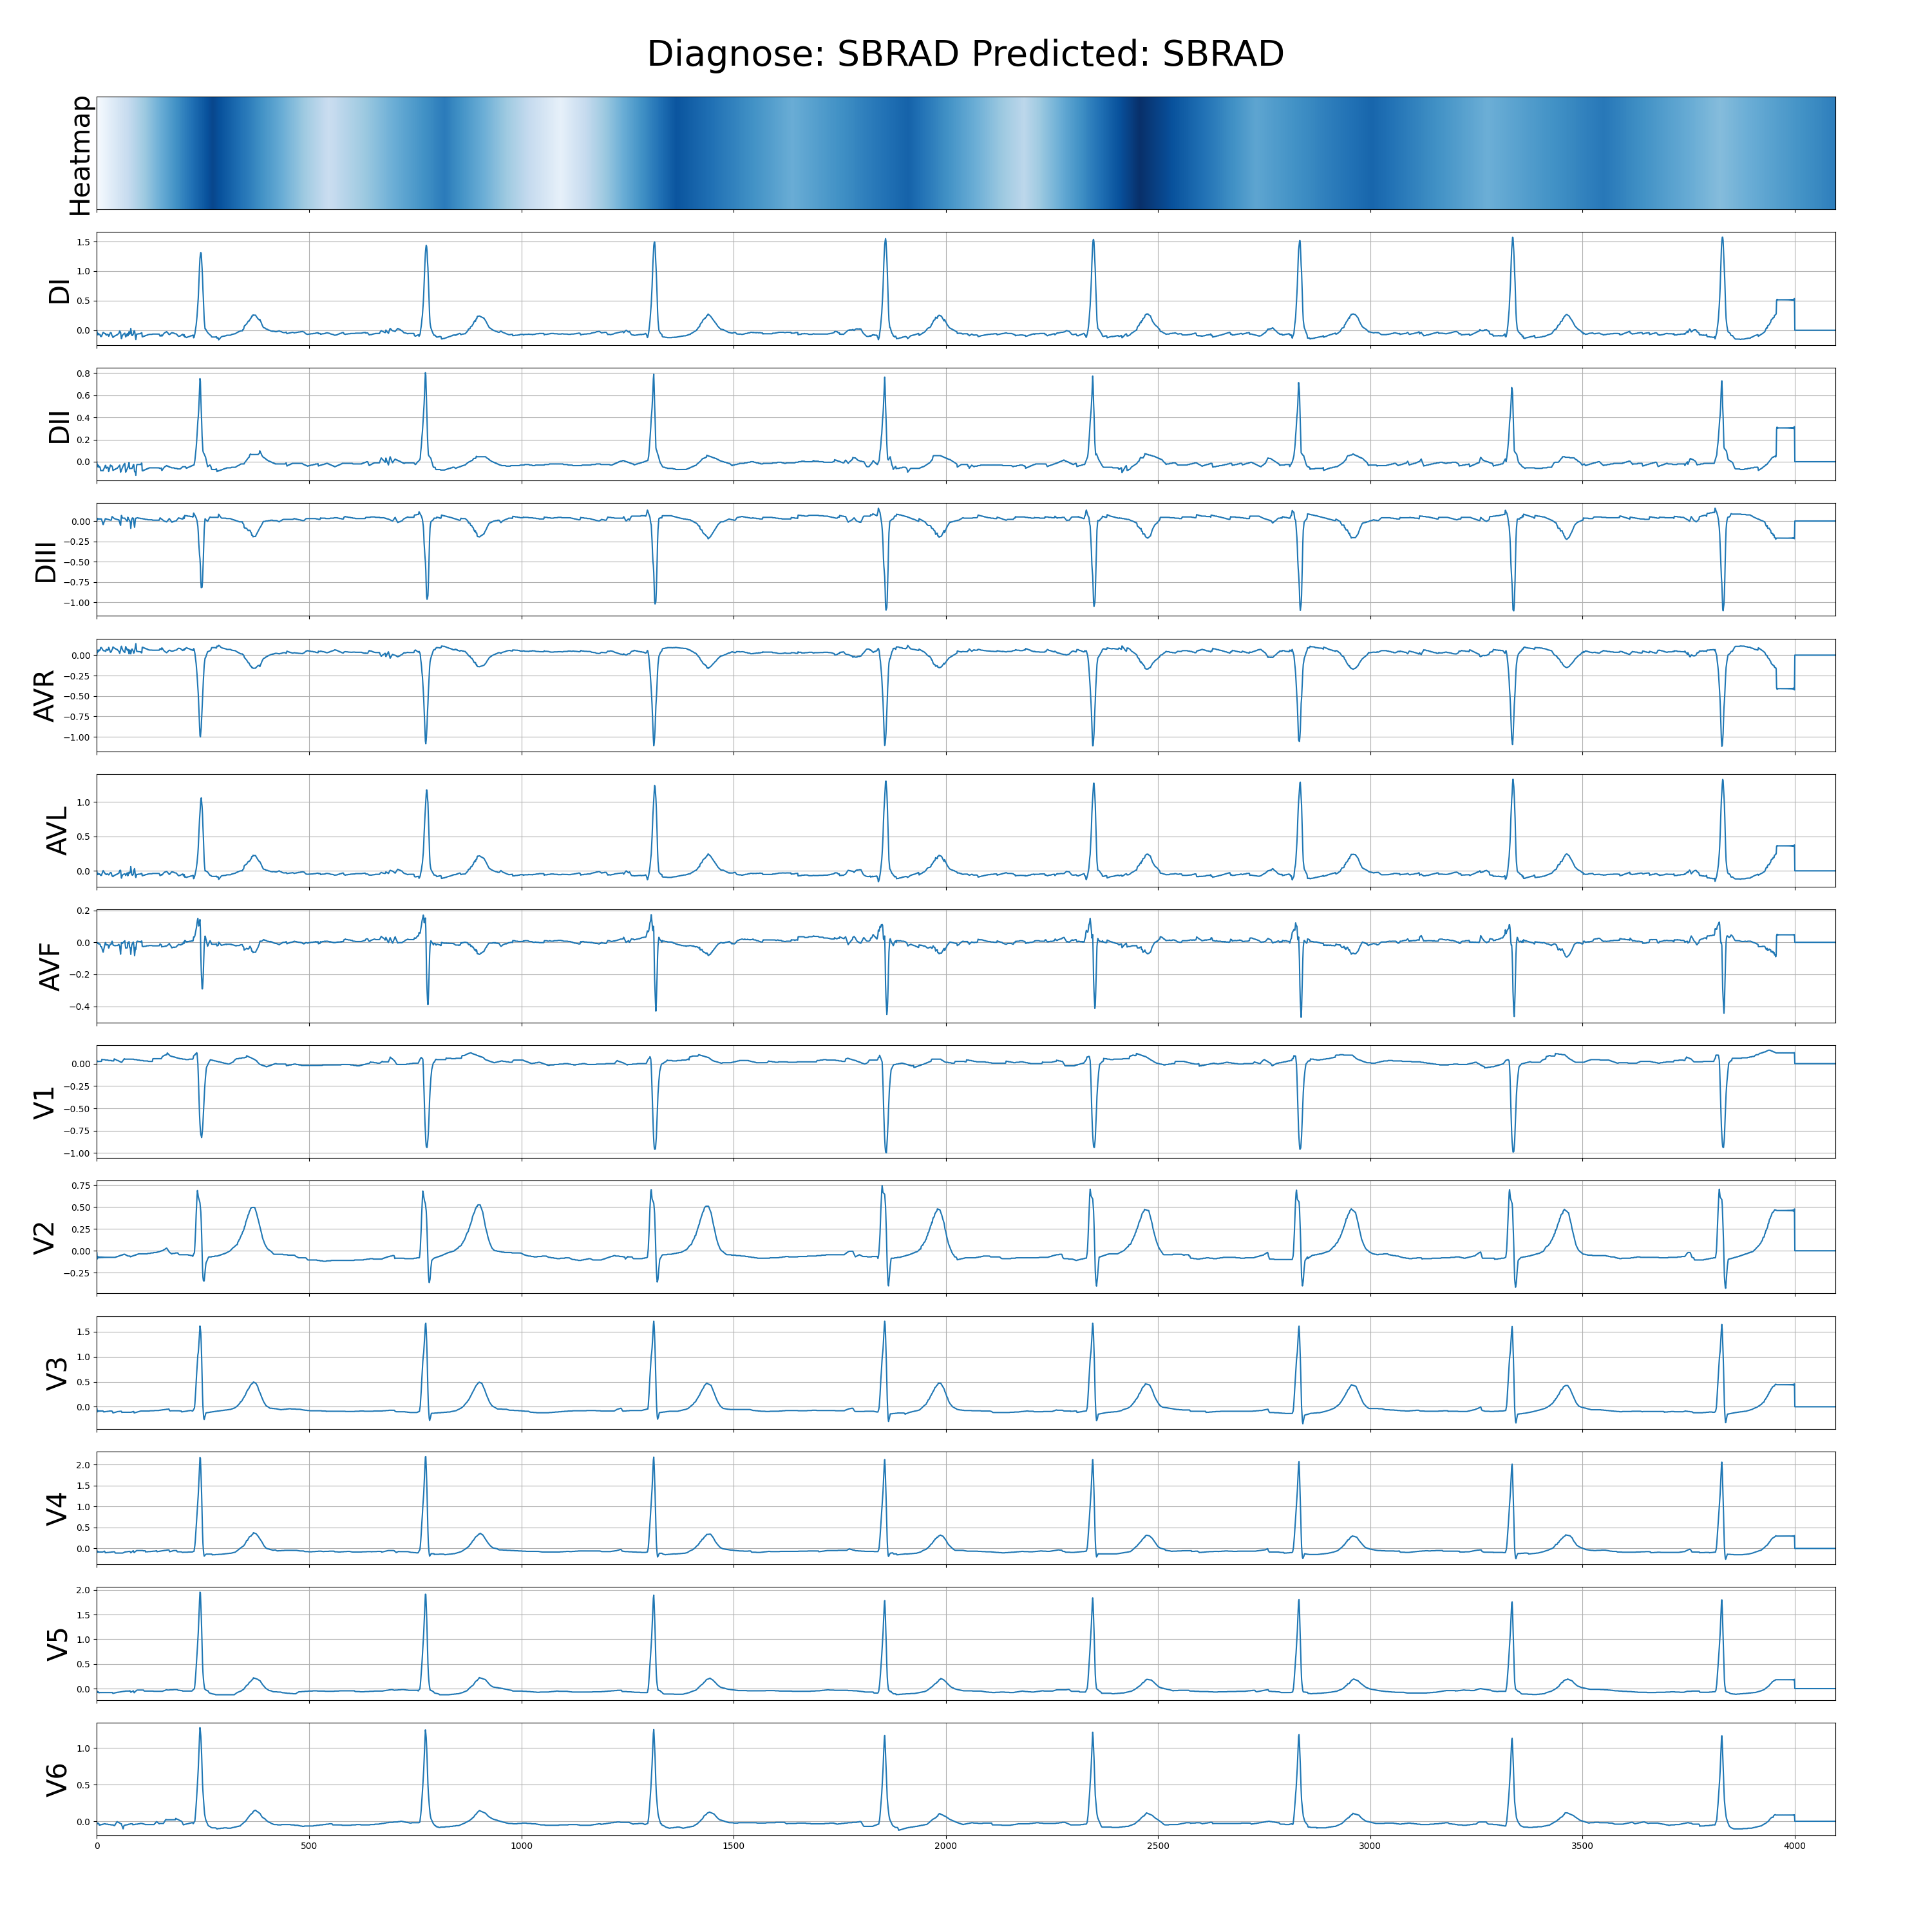
\includegraphics[width=1.1\linewidth]{\picPath/ecg_viz/19715.png}
\end{center}
  \caption{Области внимания модели для ЭКГ сигнала с диагнозом "синусовая брадикардия"}

\end{figure}
\newpage
\begin{figure}[H]
\begin{center}
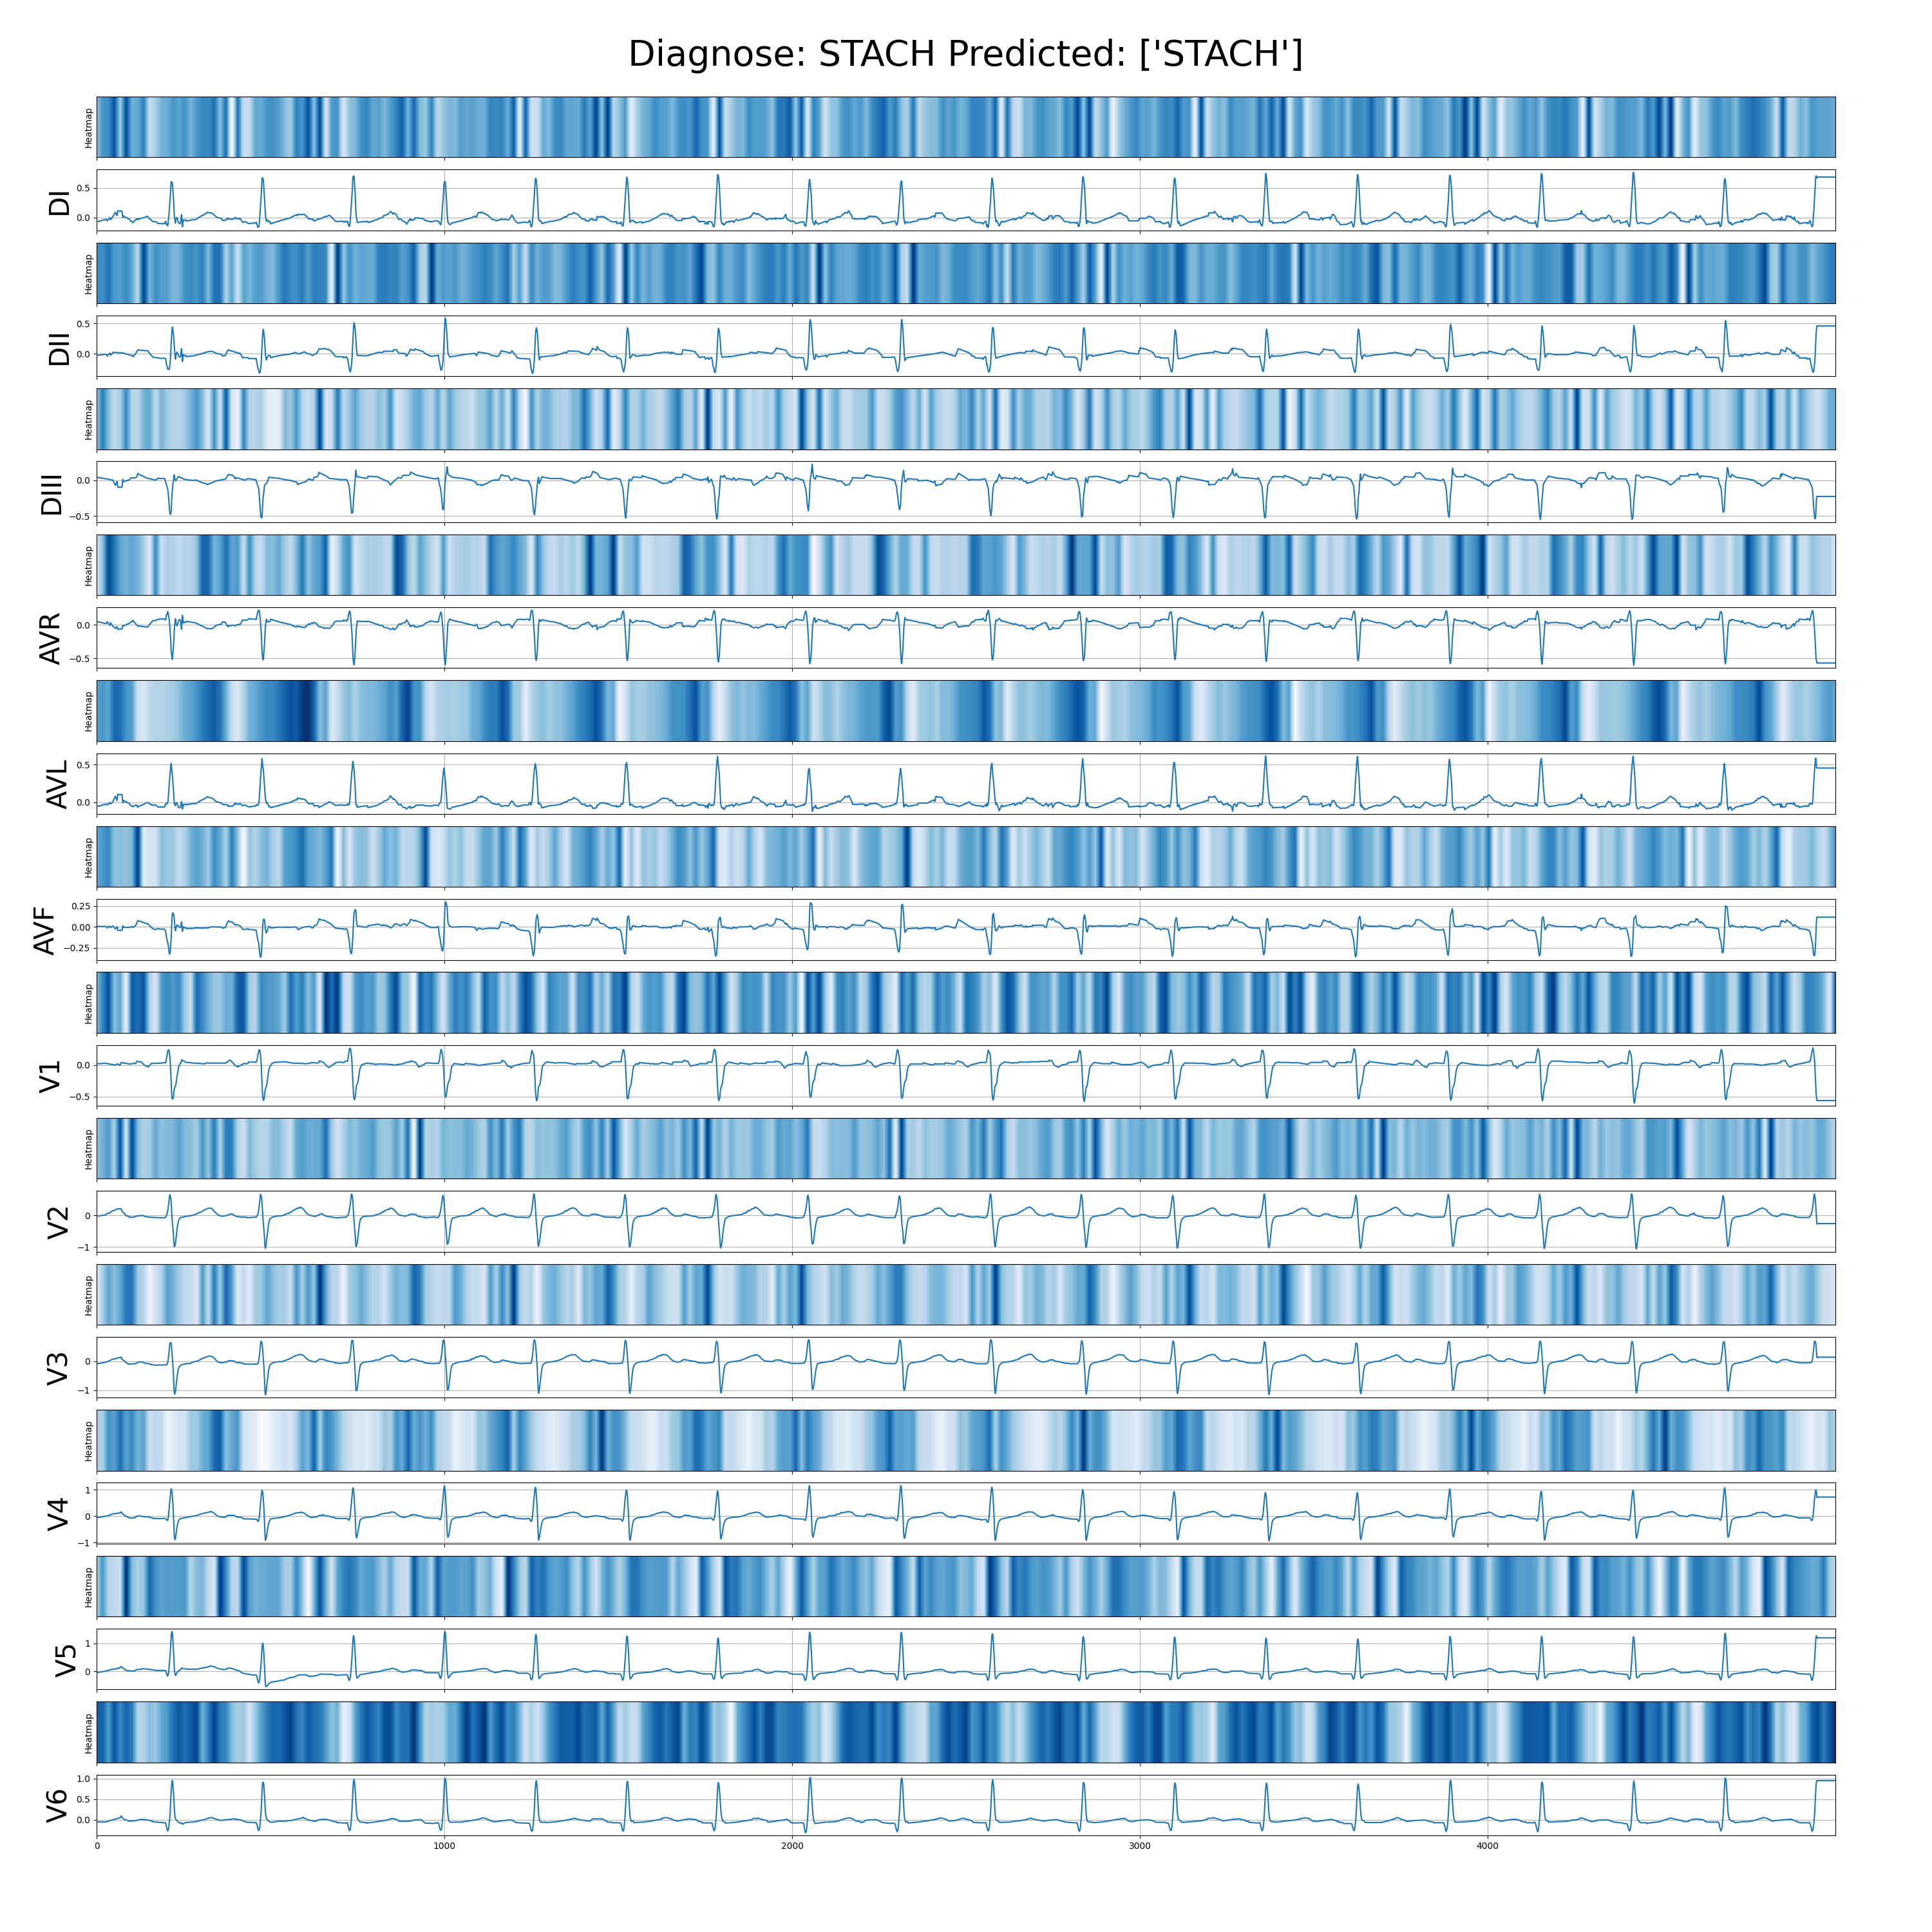
\includegraphics[width=1.1\linewidth]{\picPath/ecg_viz/21585.png}
\end{center}
  \caption{Области внимания модели для ЭКГ сигнала с диагнозом "синусовая тахикардия"}
  \label{pic:21585.png}
\end{figure}

\section{Архитектурные эксперименты: СonvAttantionNet}
\subsection{Описание архитектуры}
Недостатком визуализаций конволюционной модели resnet типа является общая карта интересов для всех каналов входного сигнала. Для того, чтобы преодолеть это ограничение, предлагается использовать новую архитектуру, реализованную в коде курсовой работы. Модель состоит из трех частей:
\begin{itemize}
\item Конволюционная часть, сосотоящиая из четырех последовательных блоков 12 групп конволюций: свертка, batchNorm слой, maxPool слой;
\item 6 последовательных слоев трансформер энкодеров, принимающие на вход, последовательно, 12 выходов групп конволюций из предыдущей части модели;
\item Классификационная часть, состоящая из одного конволюционного блока из первой части модели, соединенного с полносвязным слоем.
\end{itemize}
Первая часть представляет из себя 12 отдельных конволюционных сетей для каждого из каналов. В этой части сети входные каналы не имеют никакой информации друг о друге. Используя последнюю свертку этого блока как слой для применения GradCam можно получить 12 отдельных карт внимания сети для каждого из входных каналов. 

Вторая часть сети выполняет роль объединения результатов свертки вместе т.е. агрегирование информации раздельно по каждому из каналов. Последний слой использует один конволюционный слой для уменьшения размерности пространства и служит в качестве финального классификатора сети.


\subsection{Результаты экспериментов}
Для тренировки модели в качестве функции потерь использовался FocalLoss с парамметрами $\alpha=10, \gamma=5$, который значительно улучшил результаты обучения в сравнении со стандартной функцией потерь MSE.  В качестве алгоритма оптимизации использовался метод Adam, leaning rate=1e-6 с регуляриционным $L_2$ членом с коэффициентом 0.1. Размер батча - $256$, всего тренирока требует $250$ эпох.  Константа обучения менялась по ходу тренировки при помощи экспоненциального планировщика(Exponential Scheduler) с парамметром $\gamma=0.999$.  Спецификацию каждого из слоев можно найти в коде работы.   В результате терировки получены следующие метрики:

\chapter{Вывод}
Новая модель СonvAttantionNet сконструированна для улучшения визуализации классификации, планируется визуализация внимания сети на 6 выбранных ЭКГ сигналах. Кроме того, возможны архитектурые улучшения сети, такие как увеличение количество каналов свертки и подбор оптимальных значений размеров ядер сверток


\end{document}